\documentclass[compress]{beamer}
\usetheme{ninscblack}

\usepackage{amsmath}
\usepackage{subfigure}
\usepackage{multirow}
\usepackage{amsmath}
\usepackage{animate} 
\usepackage{moresize}
\usepackage{tabularx}
\usepackage{booktabs}
\usepackage{colortbl}
\usepackage{ulem}
\usepackage{tikz}
\usetikzlibrary{calc}
\usepackage{hyperref}

\pgfdeclarelayer{background}
\pgfdeclarelayer{foreground}
\pgfsetlayers{background,main,foreground}


\input{latex-preamble/cmddef.tex}

%\newcommand{\black}[1]{{\color{black}#1}}
\renewcommand{\emph}[1]{\textbf{#1}}
%\newcommand{\beq}[1]{\[\black{#1}\]}
     
%%%%%%%%%%%%%%%%%%%%%%%%%%%%%%%%%%%%%%%%%%%%%%%%%%%%%%%%%%%%%%%%%%%%%%%%%%%%%%%%%%%%%%%%%%
%%%%%%%%%%%%%%%%%%%%%%%%%%%%%% Title Page Info %%%%%%%%%%%%%%%%%%%%%%%%%%%%%%%%%%%%%%%%%%%
%%%%%%%%%%%%%%%%%%%%%%%%%%%%%%%%%%%%%%%%%%%%%%%%%%%%%%%%%%%%%%%%%%%%%%%%%%%%%%%%%%%%%%%%%%

\title{M/EEG source modeling}
\author{Germ{\'a}n G{\'o}mez-Herrero}
\institute{Advanced Human Neurophysiology course\\VU University Amsterdam}
\date{\today}


%%%%%%%%%%%%%%%%%%%%%%%%%%%%%%%%%%%%%%%%%%%%%%%%%%%%%%%%%%%%%%%%%%%%%%%%%%%%%%%%%%%%%%%%%%
%%%%%%%%%%%%%%%%%%%%%%%%%%%%%% Begin Your Document %%%%%%%%%%%%%%%%%%%%%%%%%%%%%%%%%%%%%%%
%%%%%%%%%%%%%%%%%%%%%%%%%%%%%%%%%%%%%%%%%%%%%%%%%%%%%%%%%%%%%%%%%%%%%%%%%%%%%%%%%%%%%%%%%%

\begin{document}

%%%%%%%%%%%%%%%%%%%%%%%%%%%%%%%%%%%%%%%%%%%%%%%%%%%%%%%%%%%%%%%%%%%%%%%%%%%%%%%%%%%%%%%%%%

\frame{
	\titlepage 
}

%%%%%%%%%%%%%%%%%%%%%%%%%%%%%%%%%%%%%%%%%%%%%%%%%%%%%%%%%%%%%%%%%%%%%%%%%%%%%%%%%%%%%%%%%%
\section{Introduction}
\subsection*{}


%%%%%%%%%%%%%%%%%%%%%%%%%%%%%%%%%%%%%%%%%%%%%%%%%%%%%% SLIDE 1

\frame{\frametitle{A bit of history}

\begin{columns}
\begin{column}{0.5\textwidth}
\tiny{Santiago Ram\'on y Cajal (1852-1934)}
\begin{figure}
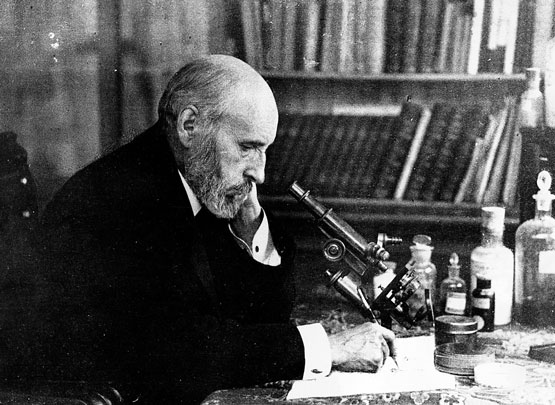
\includegraphics[width=\textwidth]{./img/ramoncajal.jpg}		
\end{figure}
\end{column}

\begin{column}{0.5\textwidth}
\tiny{The six layers of the mouse neocortex}
\begin{figure}
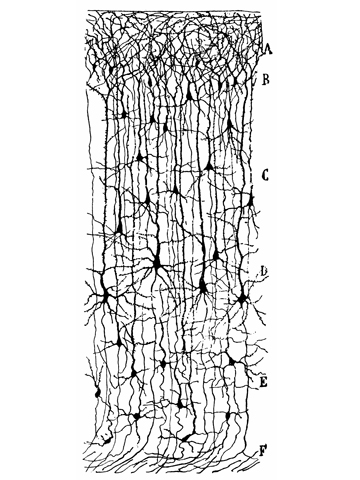
\includegraphics[width=.9\textwidth]{./img/cajalsketch.jpg}		
\end{figure}
\end{column}

\end{columns}


}

%% Notes:

% Santiago Ramon y Cajal is considered by many the father of modern neuroscience. 
% His great contribution was to provide definitive evidence for what later would
% be known as the "neuron theory". The neuron theory is really is the beginning
% of what we all know as neuroscience. Before Cajal, the central nervous system 
% was thought to be a web of continuous elements without any functional specialization.
%
% The great success of Cajal was due to his unique technical skills. To all 
% practical effects he had the best anatomical scanning technology of the time. 
% He improved a staining technology developed by Camillo Golgi which allowed him
% to draw pictures of the central nervous system with an unprecedented level of
% detail. 
%
% Cajal's anatomical studies were always presented in a functional context (Llin�s, 
% 2003). One of his most insightful hypotheses was that neurons were functionally
% polarized, that is, electrical impulses propagate from dendrites to the cell body to
% the axon. He rightly saw neurons as information processing units that make connections
% and organize into dynamic networks to accomplish their various functions. The neuron
% doctrine constitutes the basis for our understanding of the organization of the nervous
% system, giving Cajal, its main architect, the stature of scientists such as Galileo,
% Newton and Darwin (Shepherd, 1991). 

% This drawing by Santiago Ramon y Cajal first appeared in volume two, part two of 
% Cajal's Textura del Sistema Nervioso del Hombre y de los Vertebrados, published in Madrid
% in 1904. The image shows the six layers of the mouse neocortex, labeled A through F, in
% Cajal's hand. Cajal's drawings provided the foundation of modern neuroanatomy by
% showing that the nervous system is composed of individual nerve cells, as opposed to a
% web of continuous elements.


%%%%%%%%%%%%%%%%%%%%%%%%%%%%%%%%%%%%%%%%%%%%%%%%%%%%%% SLIDE 2
\frame{\frametitle{A bit of history}

'' [technique is] so important that [...] it may be stated that great discoveries are in the hands of the finest and most knowledgeable experts on one or more of the analytical methods'' (Cajal, 1899; p65). 

}


%%%%%%%%%%%%%%%%%%%%%%%%%%%%%%%%%%%%%%%%%%%%%%%%%%%%%% SLIDE 3

\frame{
\frametitle{Mapping the human brain: from structure to function}

\begin{columns}

\begin{column}{.5\textwidth}

\begin{figure}
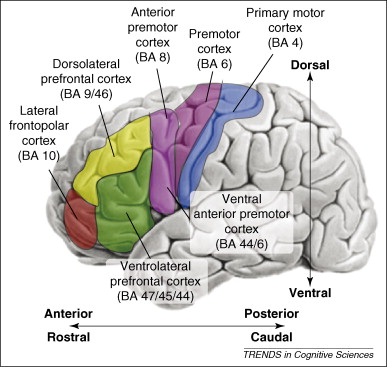
\includegraphics[width=\textwidth]{./img/frontalregions.jpg}	
\end{figure}
\tiny{D. Badre, Trends in Cognitive Sciences, 2008}
\end{column}

\begin{column}{.45\textwidth}
\begin{figure}
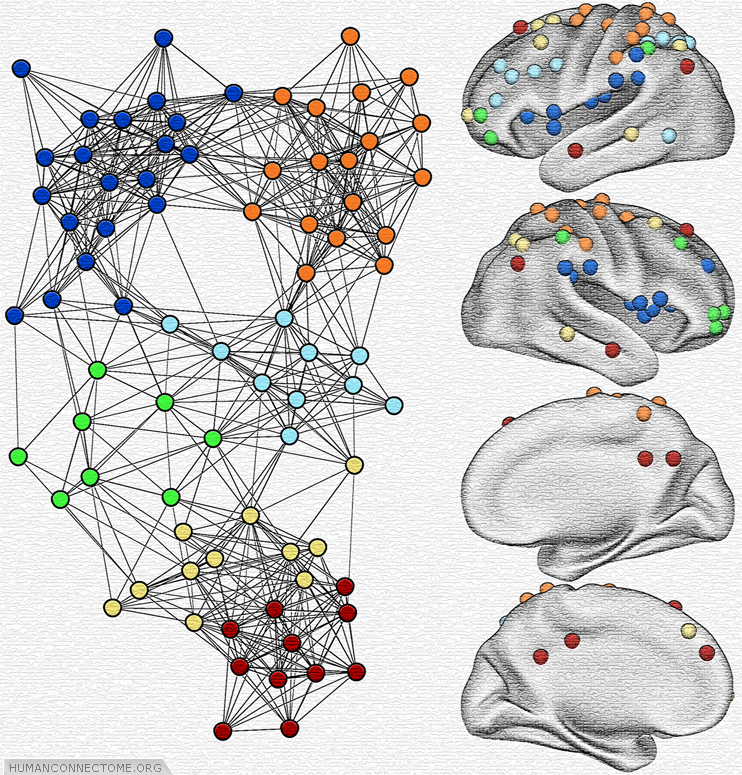
\includegraphics[width=\textwidth]{./img/connectome.png}	
\end{figure}
\tiny{Nelson et al., Neuron, 2010}
\end{column}

\end{columns}

}


%%% Notes:

%
% On the left, a schematic of major anatomical sub-divitions in the frontal lobes.
% 
%
% On the right a parcellation scheme for human left lateral parietal cortex
%
% The parietal lobe has long been viewed as a collection of architectonic and functional
% subdivisions. Though much parietal research has focused on mechanisms of visuospatial
% attention and control-related processes, more recent functional neuroimaging studies 
% of memory retrieval have reported greater activity in left lateral parietal cortex
% (LLPC) when items are correctly identified as previously studied (�old�) versus
% unstudied (�new�). These studies have suggested functional divisions within LLPC that
% may provide distinct contributions toward recognition memory judgments. Here, we define
% regions within LLPC by developing a parcellation scheme that integrates data from
% resting-state functional connectivity MRI and functional MRI. This combined approach
% results in a 6-fold parcellation of LLPC based on the presence (or absence) of
% memory-retrieval-related activity, dissociations in the profile of task-evoked time
% courses, and membership in large-scale brain networks. This parcellation should serve
% as a roadmap for  future investigations aimed at understanding LLPC function.


%%%%%%%%%%%%%%%%%%%%%%%%%%%%%%%%%%%%%%%%%%%%%%%%%%%%%% SLIDE 4

\frame{\frametitle{Functional brain imaging}


\begin{itemize}
\item Functional brain imaging techniques characterize brain function using spatiotemporal activity maps
\begin{columns}
\begin{column}{.3\textwidth}
\begin{figure}
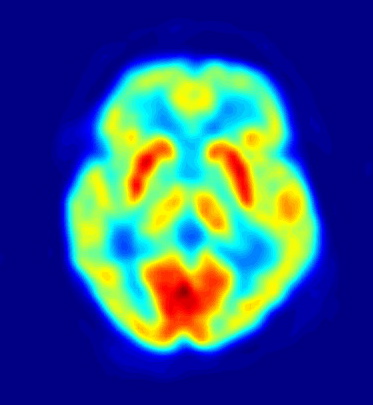
\includegraphics[width=.7\textwidth]{./img/PET.jpg}
\end{figure}
\end{column}
\begin{column}{.3\textwidth}
\begin{figure}
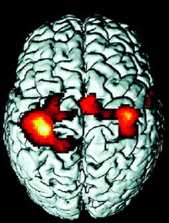
\includegraphics[width=.7\textwidth]{./img/fMRI.png}
\end{figure}
\end{column}	
\begin{column}{.3\textwidth}
\begin{figure}
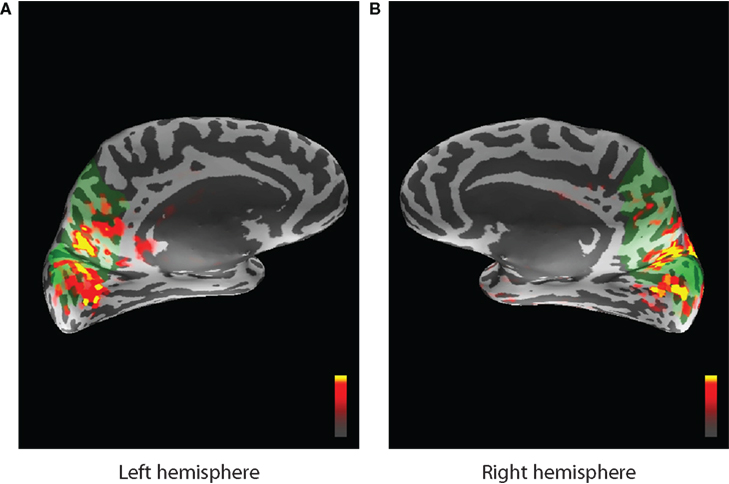
\includegraphics[trim = 2mm 10mm 32mm 2mm, clip,width=.9\textwidth]{./img/fninf-04-00114-g012.jpg}
\end{figure}
\end{column}	
\end{columns}
\vspace{.5cm} 
\item Spatial resolution is important, but...
\vspace{.5cm}
\item Temporal resolution is probably crucial
\end{itemize}


}


%%%%%%%%%%%%%%%%%%%%%%%%%%%%%%%%%%%%%%%%%%%%%%%%%%%%%% SLIDE 5

\frame{\frametitle{What are the main alternatives out there?}

\begin{center}
\vspace{-.5cm}
\begin{tikzpicture}
\node (tbl) {
\begin{tabularx}{\textwidth}{ll}
\arrayrulecolor{green}
\midrule
\multirow{4}{*}{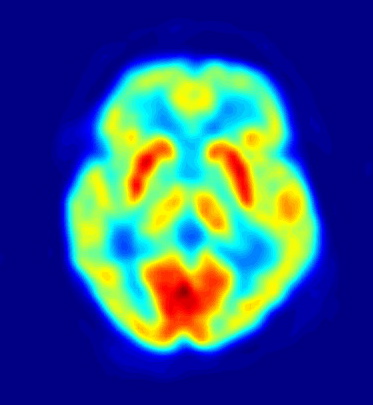
\includegraphics[height=.2\textheight]{./img/PET.jpg}} & Positron Emission Topography (PET) can be used\\
& to image metabolism with high spatial resolution\\
& ($\sim$1mm), but poor temporal resolution ($\sim$ minutes)\\
&\\
\midrule
\multirow{4}{*}{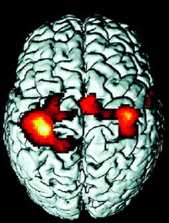
\includegraphics[height=.25\textheight]{./img/fMRI.png}} & Functional Magnetic Resonance Imaging (fMRI)\\
&can map brain hemodynamics with high spatial\\
&resolution ($\sim$1mm) but relatively poor temporal\\
& resolution ($\sim$1s)\\
&\\
\midrule

\multirow{4}{*}{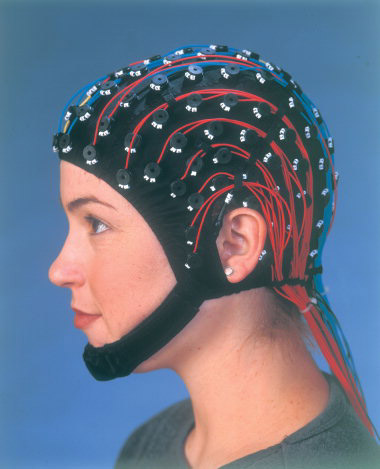
\includegraphics[height=.2\textheight]{./img/eeg2.jpg}} & Electroencephalography (EEG) and Magneto-\\
&encephalography (MEG) can track extremely fast\\
&processes ($\sim$10ms) but with poor spatial resolution\\
&\\
\midrule 
\end{tabularx}};
\end{tikzpicture}
\end{center}



}




%%%%%%%%%%%%%%%%%%%%%%%%%%%%%%%%%%%%%%%%%%%%%%%%%%%%%% SLIDE 6


\frame{\frametitle{M/EEG generation}

\begin{columns}
\begin{column}{.7\textwidth}
\begin{center}
\includegraphics<1->[width=\textwidth]{./img/neuron.png}
\end{center}
\end{column}
\begin{column}{.3\textwidth}
\begin{center}
\includegraphics<2->[width=\textwidth]{./img/dipole.pdf}
\end{center}
\end{column}
\end{columns}
}

% NOTES (from http://www.bris.ac.uk/synaptic/basics/): 

% Neurons pump out positively charged sodium ions. In addition, they pump in
% positively charged potassium ions. Thus there is a high concentration of
% sodium ions present outside the neuron, and a high concentration of potassium
% ions inside. The neuronal membrane also contains specialised proteins called 
% channels, which form pores in the membrane that are selectively permeable to 
% particular ions. Thus sodium channels allow sodium ions through the membrane 
% while potassium channels allow potassium ions through.

% Under resting conditions, the potassium channel is more permeable to potassium
% ions than the sodium channel is to sodium ions. So there is a slow outward leak
% of potassium ions that is larger than the inward leak of sodium ions. This 
% means that the membrane has a charge on the inside face that is negative 
% relative to the outside, as more positively charged ions flow out of the neuron
% than flow in. This difference in the concentrations of ions on either side of 
% the membrane gives rise to the membrane potential and the membrane is said to be
% polarised. 

% However, if the sodium channels are opened, positively charged sodium ions flood
% into the neuron, and making the inside of the cell momentarily positively 
% charged - the cell is said to be depolarized. This has the effect of opening the
% potassium channels, allowing potassium ions to leave the cell. Thus, there is 
% first an influx of sodium ions (leading to massive depolarization) followed by 
% a rapid efflux of potassium ions from the neuron (leading to repolarisation). 
% Excess ions are subsequently pumped in/out of the neuron. 

% Neurons communicate at structures called synapses in a process called synaptic
% transmission. The synapse consists of the two neurons, one of which is sending
% information to the other. The sending neuron is known as the pre-synaptic neuron
% (i.e. before the synapse) while the receiving neuron is known as the 
% post-synaptic neuron (i.e. after the synapse). Although the flow of information
% around the brain is achieved by electrical activity, communication between 
% neurons is a chemical process. When an action potential reaches a synapse, pores
% in the cell membrane are opened allowing an influx of calcium ions (positively
% charged calcium atoms) into the pre-synaptic terminal. This causes a small 
% 'packet' of a chemical neurotransmitter to be released into a small gap between 
% the two cells, known as the synaptic cleft. The neurotransmitter diffuses across
% the synaptic cleft and interacts with specialized proteins called receptors that
% are embedded in the post-synaptic membrane. These receptors are ion channels that
% allow certain types of ions (charged atoms) to pass through a pore within their
% structure. The pore is opened following interaction with the neurotransmitter 
% allowing an influx of ions into the post-synaptic terminal, which is propagated
% along the dendrite towards the soma.


%%%%%%%%%%%%%%%%%%%%%%%%%%%%%%%%%%%%%%%%%%%%%%%%%%%%%% SLIDE 7


\frame{\frametitle{M/EEG generation}

\begin{itemize}
\item \small Synchronously activated large pyramidal 
cortical neurons are believed to be the main MEG/EEG generators
\vspace{.2cm}
\item \small A synchronous cortical patch 5mm x 5mm 
would probably yield enough net current to be measurable at the scalp
\end{itemize}

\begin{center}
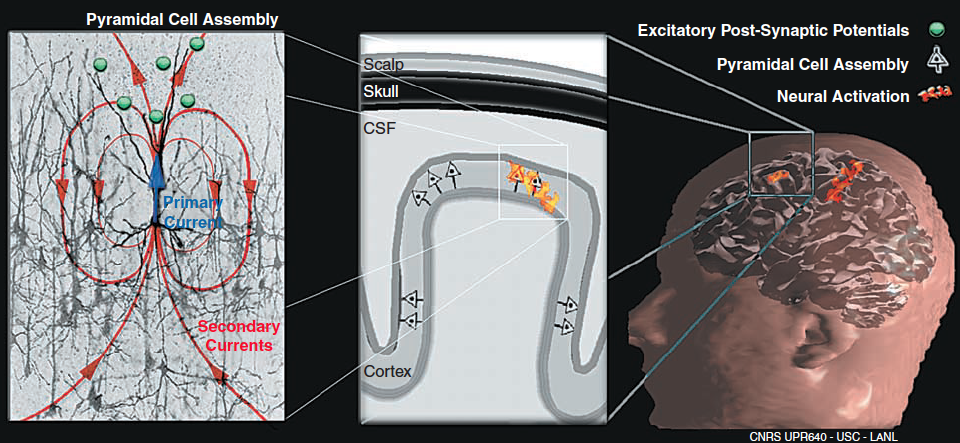
\includegraphics[width=.9\textwidth]{./img/eegmeg-generation.png}
\end{center}
}

% NOTES: 
%
% Macrocolumns of tens of thousands of neurons.
%
% The main reason is that such cortical columns have large dendritic trunks
% locally oriented in parallel and pointing perpendicularly to the cortical
% surface. 
%
% The currents associated with the EPSPs generated among their dendrites are 
% believed to be at the source of most of the signals detected in MEG and EEG
% because they typically last longer (up to 100 ms) than the rapidly firing 
% action potentials (2ms) traveling along the axons of excited neurons.
%
% Some approximate calculations suggest that what we are seeing with EEG/MEG
% is the cumulative summation of millions of synaptic juntions in a relatively
% small region
%
% Nominal calculations of neuronal density and cortical thickness suggest that
% the cortex has a macrocellular current density on the order of 100nA/mm2
% If we assume the cortex is about 4 mm thick, then a small patch 5x5mm would
% yield the necessary current to be measurable at the scalp



%%%%%%%%%%%%%%%%%%%%%%%%%%%%%%%%%%%%%%%%%%%%%%%%%%%%%% SLIDE 8


\frame{\frametitle{M/EEG sources}

\begin{itemize}
\item A relatively compact cluster of neurons firing in synchrony so that the temporal variations of their average EPSPs are measurable at the scalp
\vspace{.2cm}
\item The average time course of those EPSPs is what we call the \emph{source activation}
\vspace{.2cm}
\item A single EEG source can be modeled as one dipole or as multiple dipoles having the same temporal pattern of activation (possibly scaled)
\end{itemize}

}

%%%%%%%%%%%%%%%%%%%%%%%%%%%%%%%%%%%%%%%%%%%%%%%%%%%%%% SLIDE 9
\frame{\frametitle{M/EEG sources}

\begin{center}
\animategraphics[autoplay,loop,width=5cm]{20}{./animated/eegsource/i}{0}{179}
\end{center}
}



%%%%%%%%%%%%%%%%%%%%%%%%%%%%%%%%%%%%%%%%%%%%%%%%%%%%%% SLIDE 11


\frame{\frametitle{What is the actual spatial resolution of scalp M/EEG?}
	\begin{itemize}
	\item  Depends on the characteristics of the underlying EEG sources
	\vspace{.3cm}
	\item It is fundamentally limited by two factors:
	\begin{itemize}
	\item The number of measurements
	\item \emph{The inherent ambiguity of the M/EEG inverse problem}
	\end{itemize}
	\vspace{.3cm}
	\item Hopefully of the order of 1-2cm
	\end{itemize}
	
}




%%%%%%%%%%%%%%%%%%%%%%%%%%%%%%%%%%%%%%%%%%%%%%%%%%%%%% SLIDE 12-13


\frame{\frametitle{The M/EEG source modeling problem}

\begin{columns}
\begin{column}{6cm}
We want to find out:
\vspace{.2cm}
\begin{itemize}
\item The number of sources
\item Source activation patterns
\item Source spatial extents
\end{itemize}
\end{column}
\begin{column}{5cm}

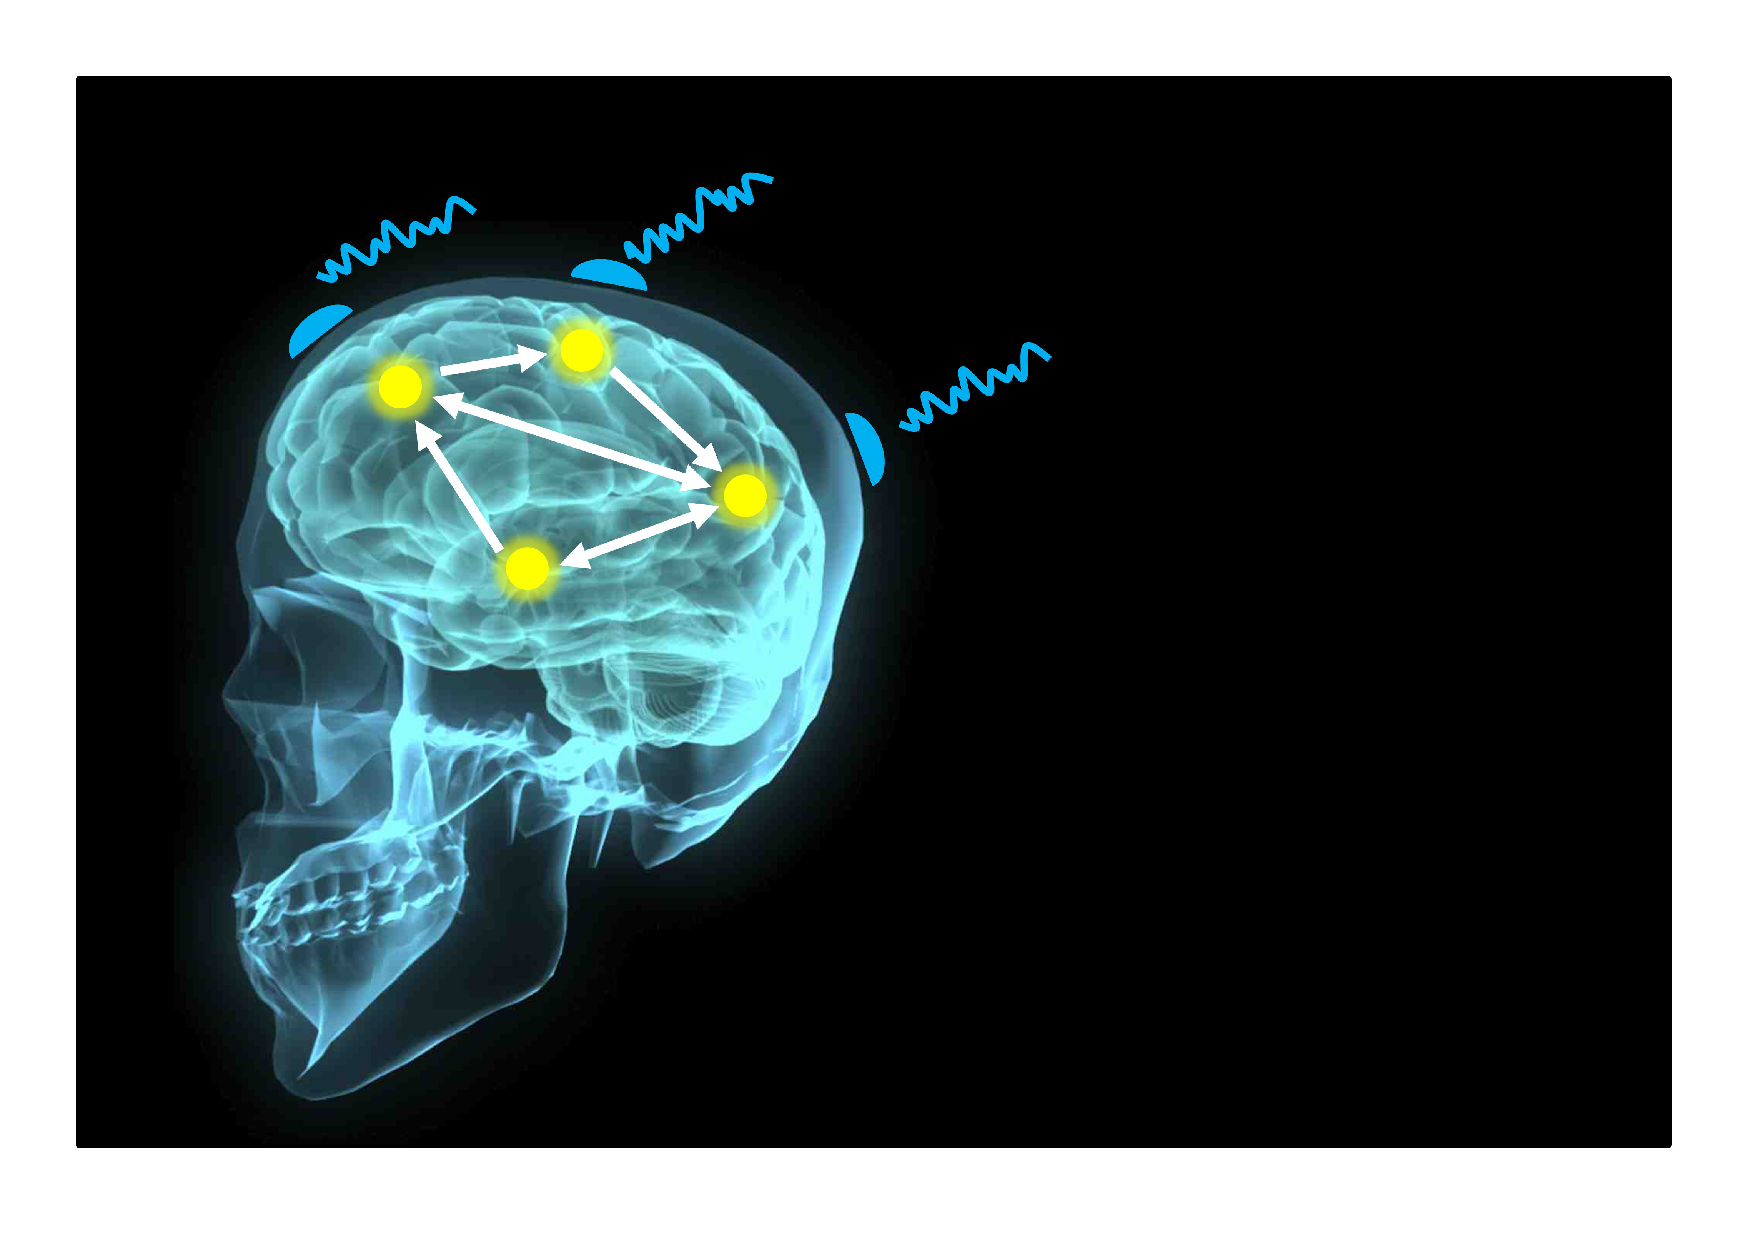
\includegraphics[width=\textwidth,trim = 3cm 2cm 9cm 2cm,clip]{./img/head.pdf}

\end{column}

\end{columns}

}


\frame{\frametitle{The M/EEG source modeling problem}
\begin{columns}
\begin{column}{6cm}
\begin{block}{How do we get there from here?}
\animategraphics[autoplay,loop,width=5cm]{5}{./animated/sim5/sim5}{1}{100}
\end{block}
\end{column}
\begin{column}{5cm}

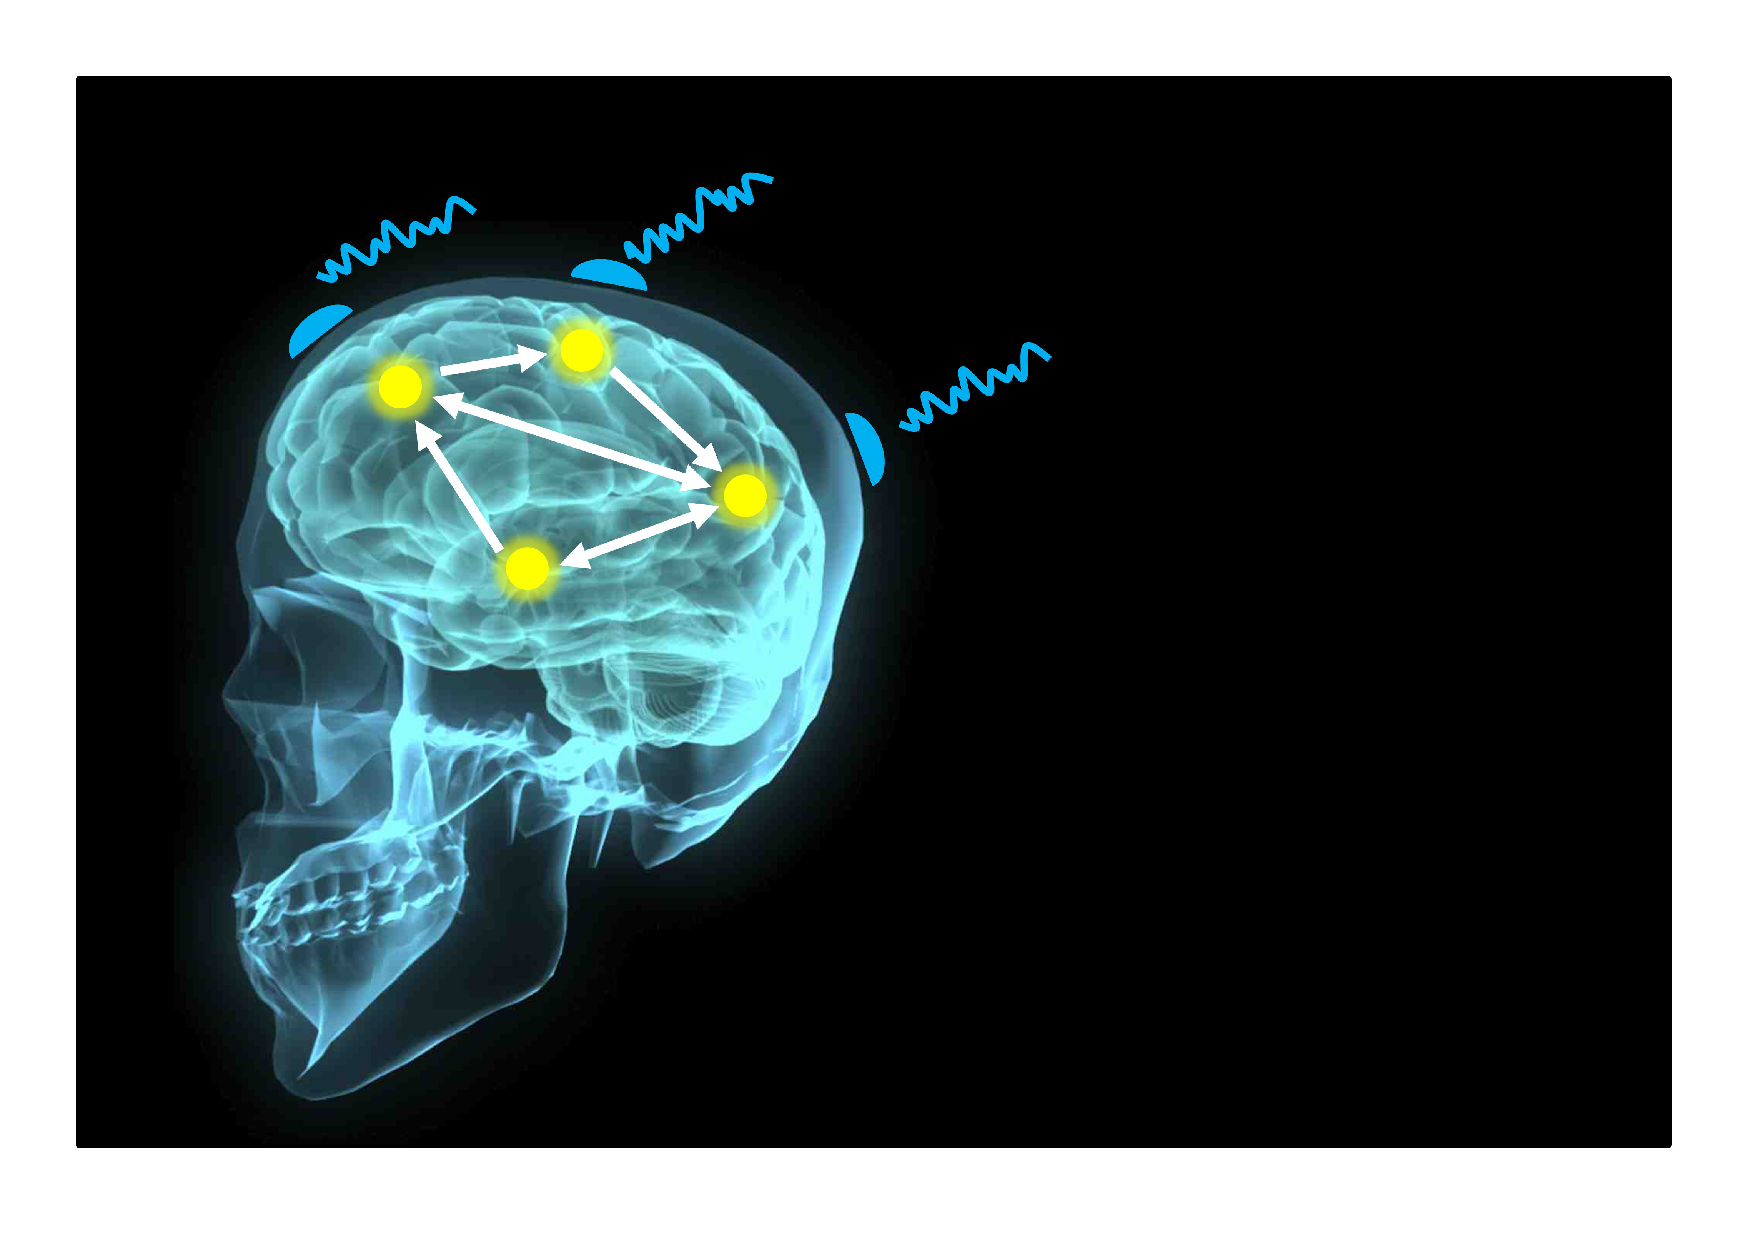
\includegraphics[width=\textwidth,trim = 3cm 2cm 9cm 2cm,clip]{./img/head.pdf}

\end{column}

\end{columns}

}


%%%%%%%%%%%%%%%%%%%%%%%%%%%%%%%%%%%%%%%%%%%%%%%%%%%%%%%%%%%%%%%%% SECTION: FORWARD PROBLEM


\section{The forward problem}
\subsection*{}

%%%%%%%%%%%%%%%%%%%%%%%%%%%%%%%%%%%%%%%%%%%%%%%%%%%%%% SLIDE 14


\frame{\frametitle{The forward electromagnetic problem}
Maxwell's laws of electromagnetism:
\begin{eqnarray}
\text{Gauss' law for electricity:}& \displaystyle \cint{\vec{E}\cdot\dA}&=\frac{Q_{enc}}{\eps0}\nonumber\\
\text{Gauss' law for magnetism:}& \displaystyle \cint{\vec{B}\cdot\dA}&=0\nonumber\\
\text{Faraday's law:}& \displaystyle\oint{\vec{E}\cdot\ds}&=-\frac{\dphib}{\dt}\nonumber\\
\text{Ampere-Maxwell law:}& \displaystyle\oint{\vec{B}\cdot\ds}&=\muz\eps0\frac{\dphie}{\dt}+\muz i_{enc}\nonumber
\end{eqnarray}

\vspace{1cm}
\tiny{Note: No need of knowing these for this course!}

}


%%%%%%%%%%%%%%%%%%%%%%%%%%%%%%%%%%%%%%%%%%%%%%%%%%%%%% SLIDE 15


\frame{\frametitle{The forward electromagnetic problem}

\begin{itemize}
\item Fortunately, for slowly varying current generators (e.g. for M/EEG frequencies), the solution to Maxwell's equations for a current dipole is just a \emph{linear and instantaneous} map:
\end{itemize}

\[
\underbrace{
\left[
\begin{array}{c}
v_1\\
v_2\\ 
\vdots\\
v_K\\
\end{array}
\right]}_{\textrm{scalp potential}}=
\underbrace{
\left[
\begin{array}{ccc}
a_{1x} & a_{1y} & a_{1z}\\
a_{2x} & a_{2y} & a_{2z}\\
\vdots & &\\
a_{Kx} & a_{Ky} & a_{Kz}\\
\end{array}
\right]}_{\textrm{leadfield}}
\underbrace{
\left[
\begin{array}{c}
q_x\\
q_y\\ 
q_z\\
\end{array}
\right]
}_{\textrm{dipole}}
\]


}


%%%%%%%%%%%%%%%%%%%%%%%%%%%%%%%%%%%%%%%%%%%%%%%%%%%%%% SLIDE 16


\frame{\frametitle{The forward electromagnetic problem}

\begin{itemize}
\item For convenience, we can also express the transformation from a dipolar current source to scalp potentials like this:
\end{itemize}

\[
\underbrace{
\left[
\begin{array}{c}
v_1\\
\vdots\\
v_K\\
\end{array}
\right]}_{\textrm{scalp potential}}=
\underbrace{
\left[
\begin{array}{ccc}
a_{1x} & a_{1y} & a_{1z}\\
\vdots & &\\
a_{Kx} & a_{Ky} & a_{Kz}\\
\end{array}
\right]}_{\textrm{leadfield}}
\underbrace{
\left[
\begin{array}{c}
j_x\\
j_y\\ 
j_z\\
\end{array}
\right]
}_{\textrm{orientation}}
\underbrace{
m
}_{\textrm{magnitude}}
\]
\begin{center}
\boxed{
\v = \a(x,y,z, j_{x}, j_y, j_z)m
}
\end{center}


where $\a(x,y,z, j_x, j_y, j_z)$ is a $K\times 1$ vector of gain coefficients. Sometimes we will also refer to it as the \emph{source leadfield}

}





%%%%%%%%%%%%%%%%%%%%%%%%%%%%%%%%%%%%%%%%%%%%%%%%%%%%%% SLIDE 17,18


\frame{\frametitle{Source leadfield / topography / ''gain vector''}

\begin{columns}
\begin{column}{5cm}
A radial superficial dipole
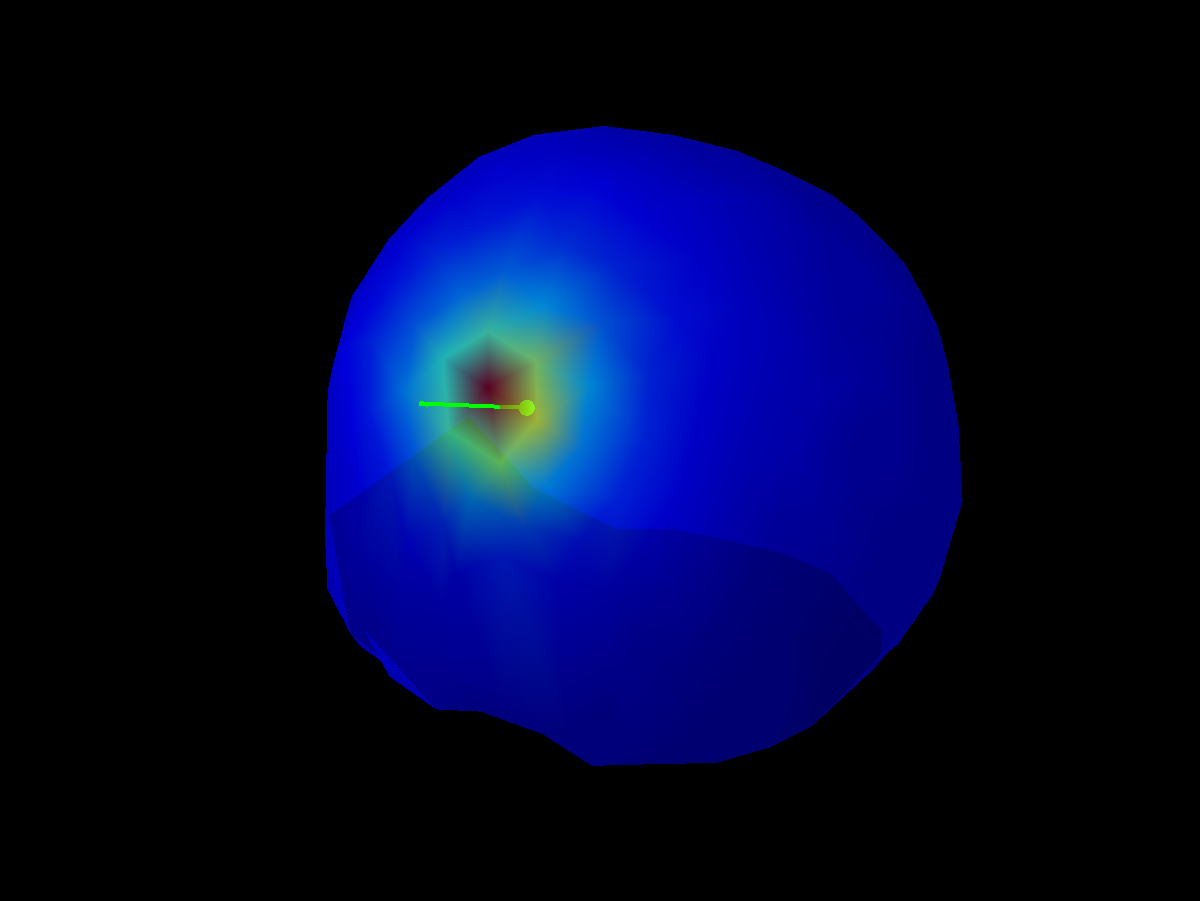
\includegraphics[width=\textwidth]{./img/dipole-leadfield-radial-superficial.png}

\end{column}
\begin{column}{5cm}
A radial deep dipole
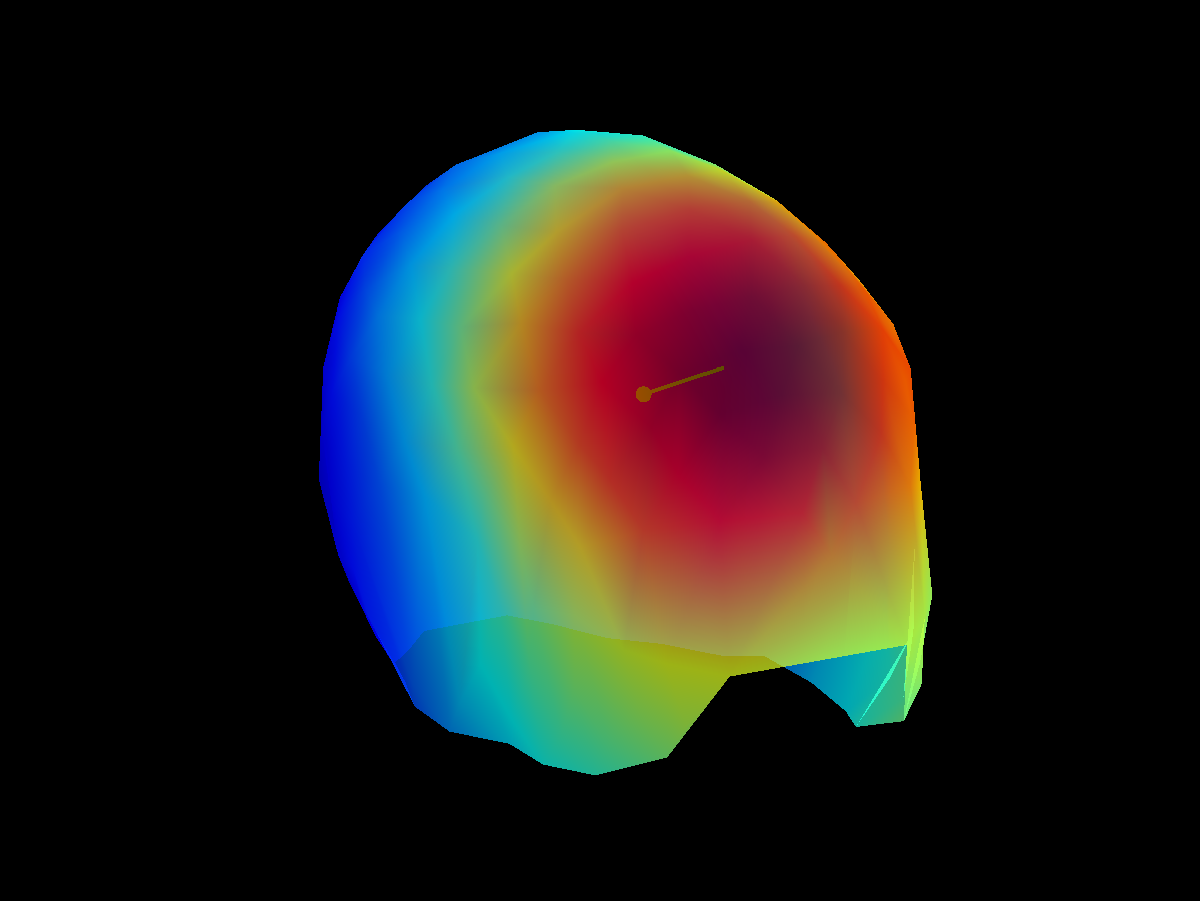
\includegraphics[width=\textwidth]{./img/dipole-leadfield-radial-deep.png}

\end{column}

\end{columns}

\[
\left[
\begin{array}{c}
v_1\\
v_2\\ 
\vdots\\
v_K\\
\end{array}
\right]=
\left[
\begin{array}{c}
a_1\\
a_2\\
\vdots\\
a_K\\
\end{array}
\right]m
\]


}

\frame{\frametitle{Source leadfield or ''gain vector''}

\begin{columns}
\begin{column}{5cm}
A tangential superficial dipole
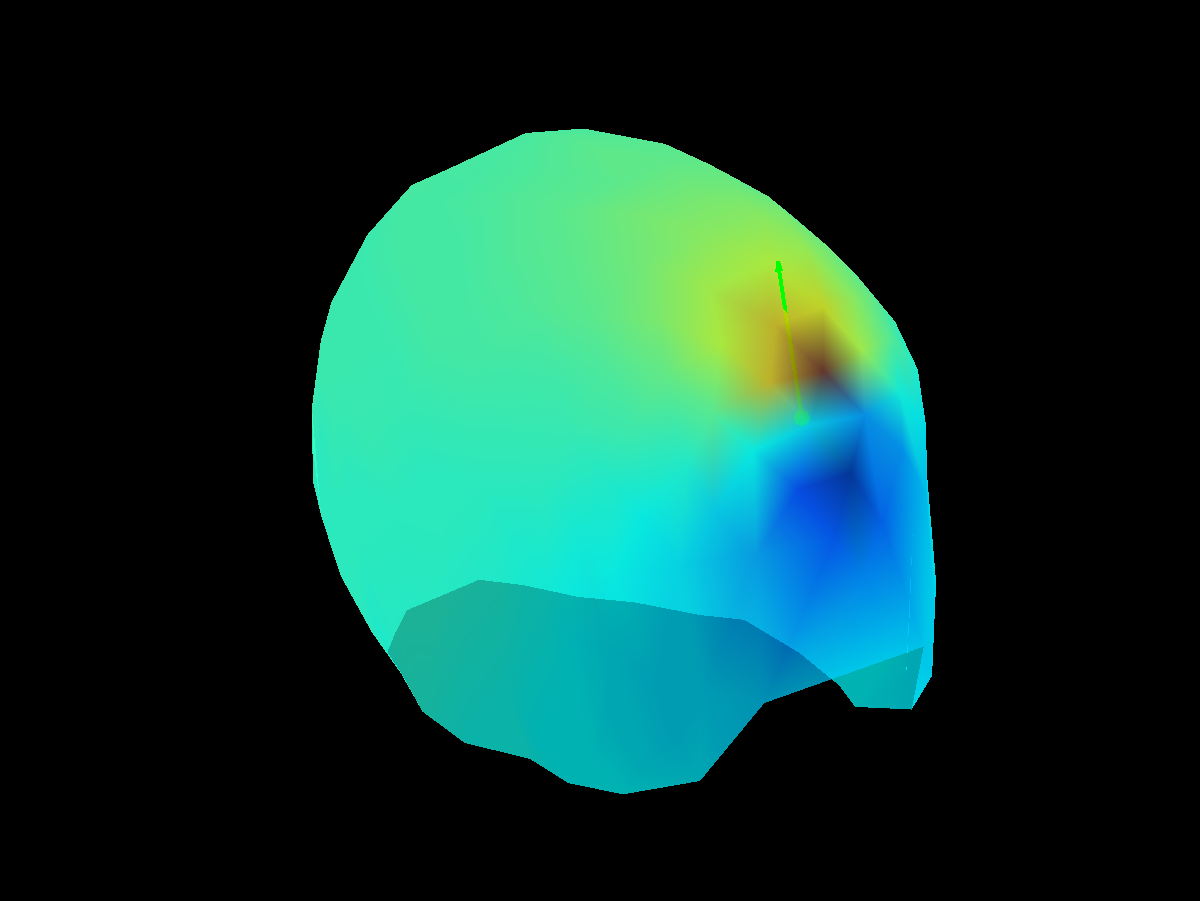
\includegraphics[width=\textwidth]{./img/dipole-leadfield-tangential-superficial.png}

\end{column}
\begin{column}{5cm}
A tangential deep dipole
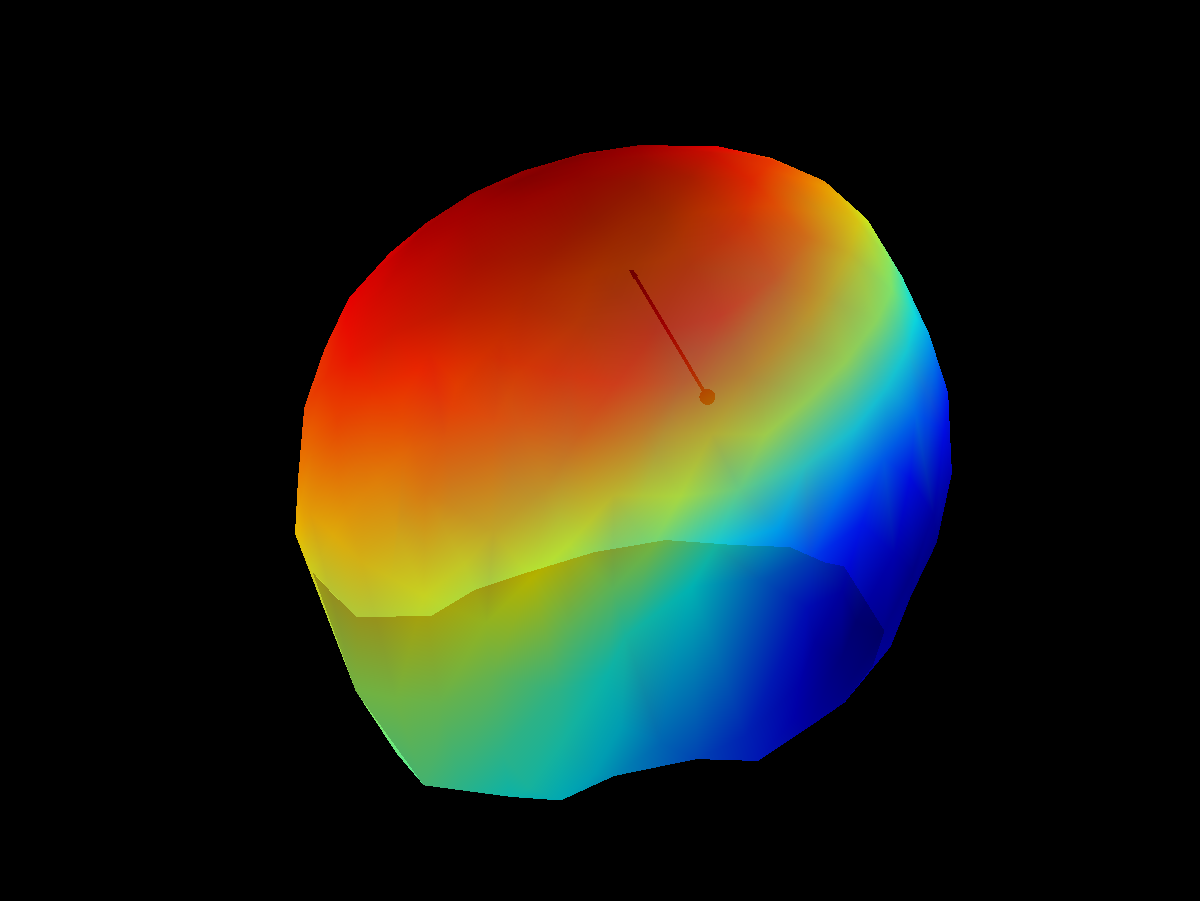
\includegraphics[width=\textwidth]{./img/dipole-leadfield-tangential-deep.png}

\end{column}

\end{columns}

\[
\left[
\begin{array}{c}
v_1\\
v_2\\ 
\vdots\\
v_K\\
\end{array}
\right]=
\left[
\begin{array}{c}
a_1\\
a_2\\
\vdots\\
a_K\\
\end{array}
\right]m
\]


}









%%%%%%%%%%%%%%%%%%%%%%%%%%%%%%%%%%%%%%%%%%%%%%%%%%%%%% WHAT ABOUT TIME VARIATION?


\frame{\frametitle{What about time variation?}


\begin{columns}

\begin{column}{.2\textwidth}
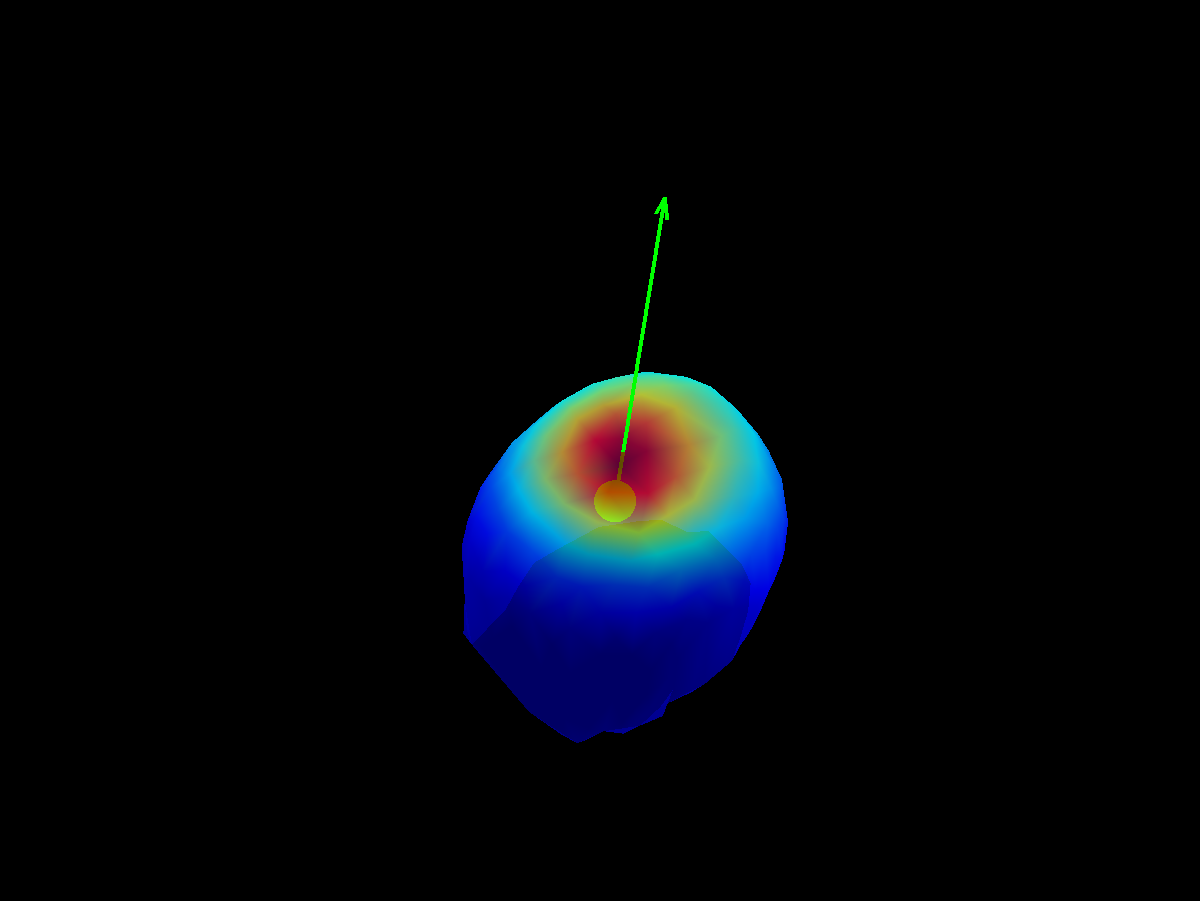
\includegraphics[width=\textwidth,trim=7cm 3cm 7cm 2cm,clip]{./img/source-time1.png}

$t=0$
\end{column}

\begin{column}{.2\textwidth}
\vspace{.6cm}
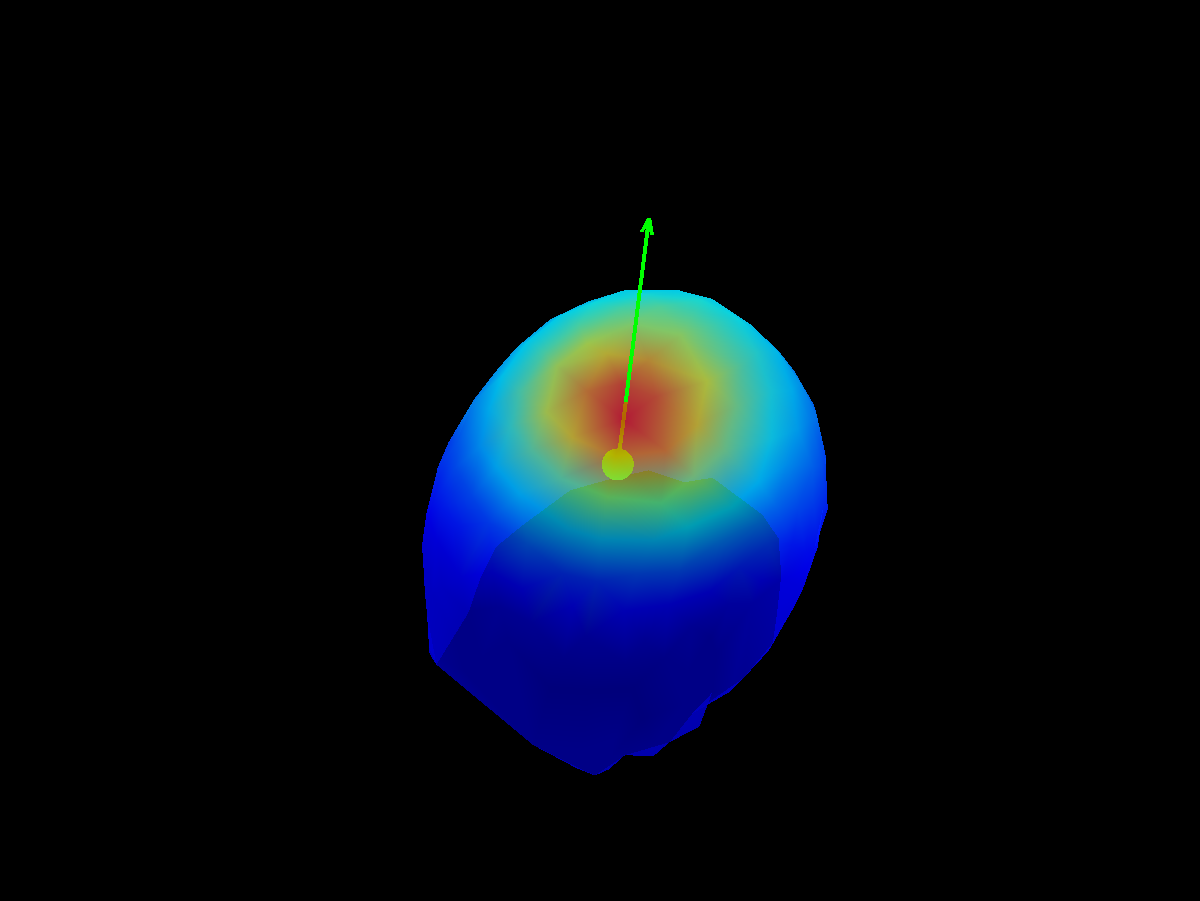
\includegraphics[width=\textwidth,trim=6.5cm 3cm 6cm 2cm,clip]{./img/source-time2.png}

$t=1$
\end{column}

\begin{column}{.2\textwidth}
\vspace{1.5cm}
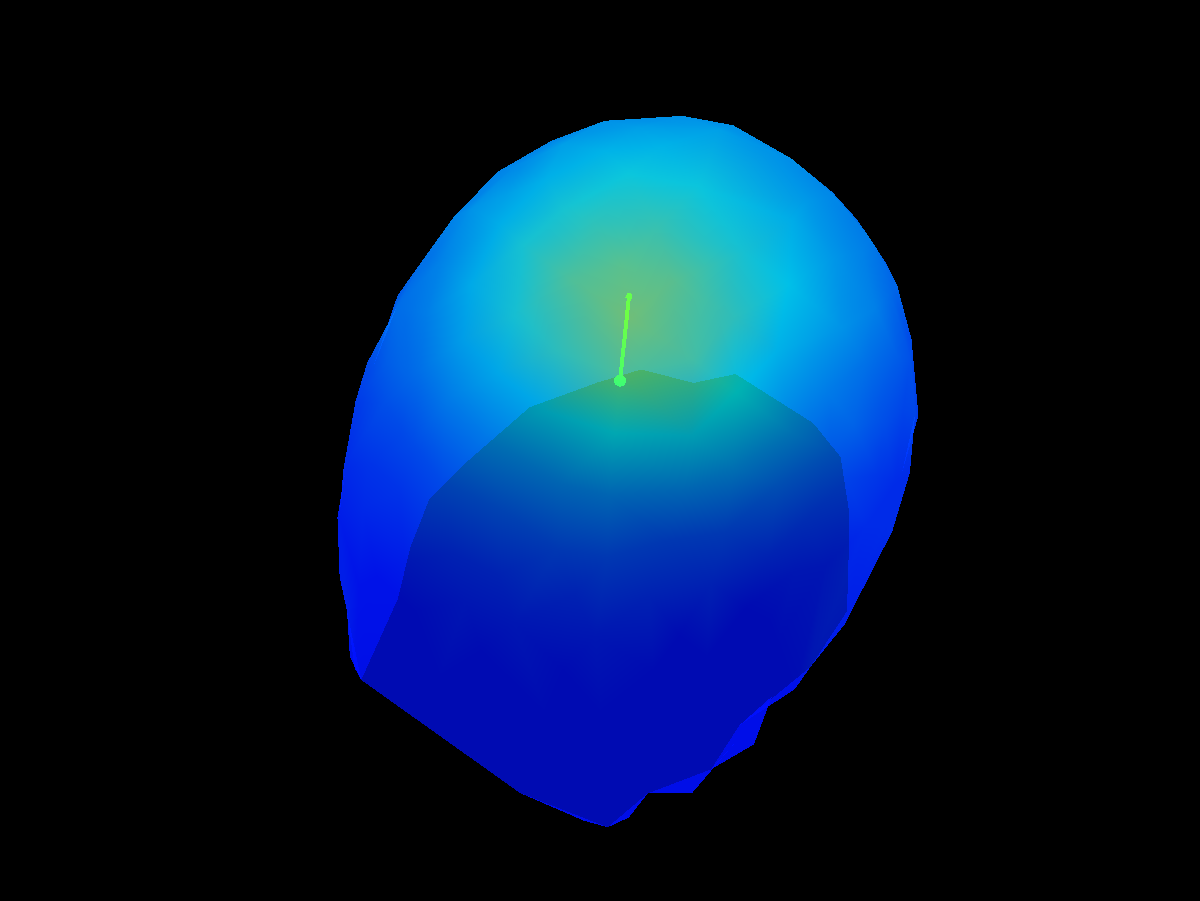
\includegraphics[width=\textwidth,trim=5cm 3cm 4cm 2cm,clip]{./img/source-time3.png}

$t=2$
\end{column}

\begin{column}{.2\textwidth}
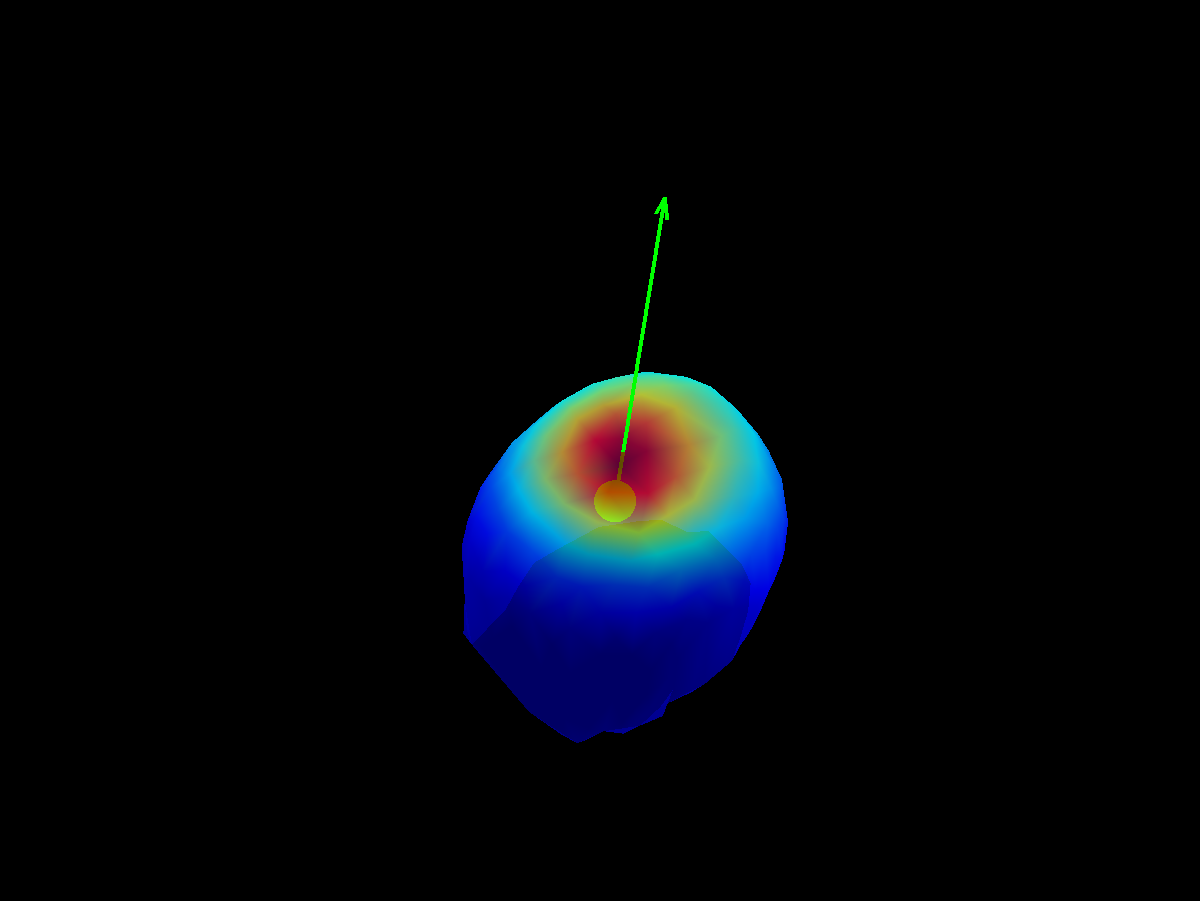
\includegraphics[width=\textwidth,trim=7cm 3cm 7cm 2cm,clip]{./img/source-time1.png}

$t=3$
\end{column}

\end{columns}



}


%%%%%%%%%%%%%%%%%%%%%%%%%%%%%%%%%%%%%%%%%%%%%%%%%%%%%% SOURCE FIELDS ARE ADDITIVE


\frame{\frametitle{Source fields are additive}

\begin{columns}
\begin{column}{3.5cm}
1 dipole (6 mm deep)
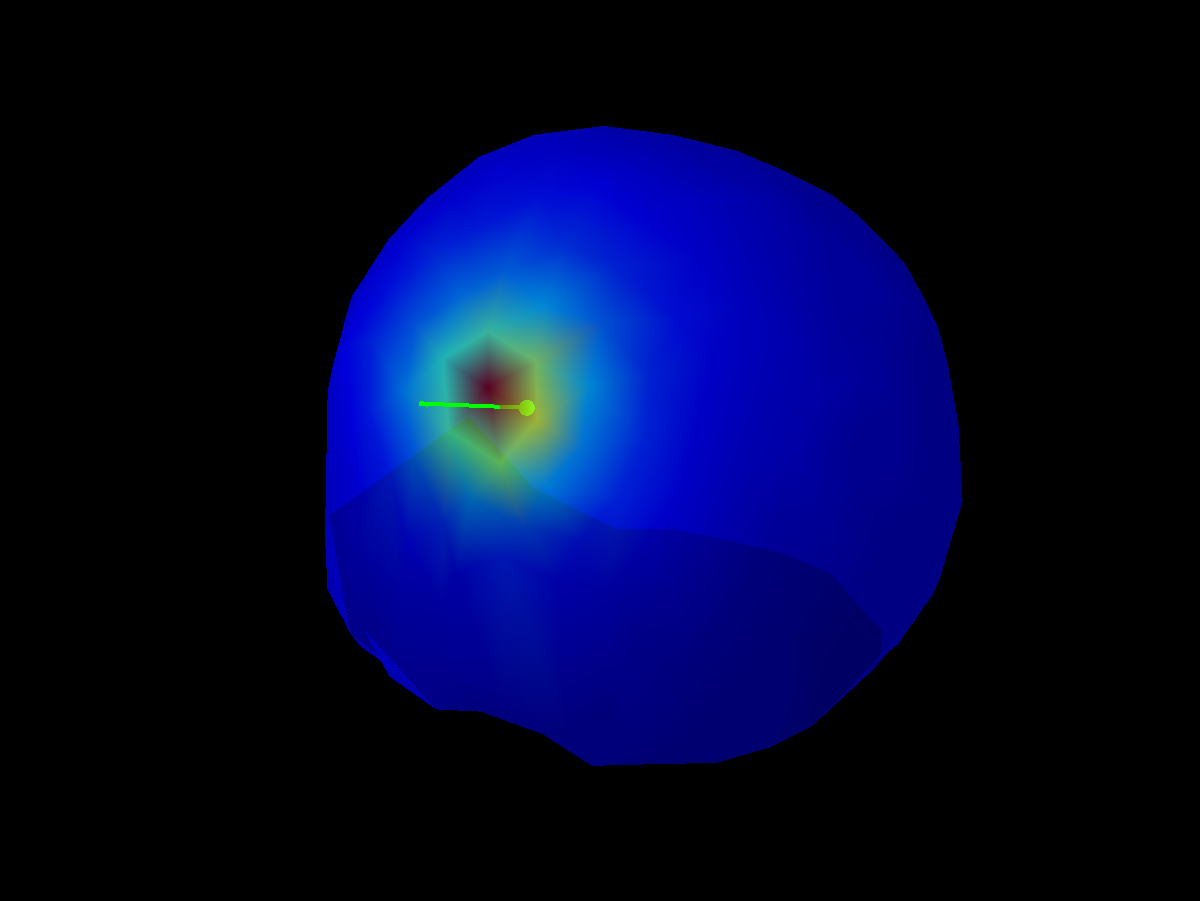
\includegraphics[width=1.2\textwidth]{./img/dipole-leadfield-radial-superficial.png}

\end{column}
\begin{column}{3.5cm}
1 dipole (2mm deep)
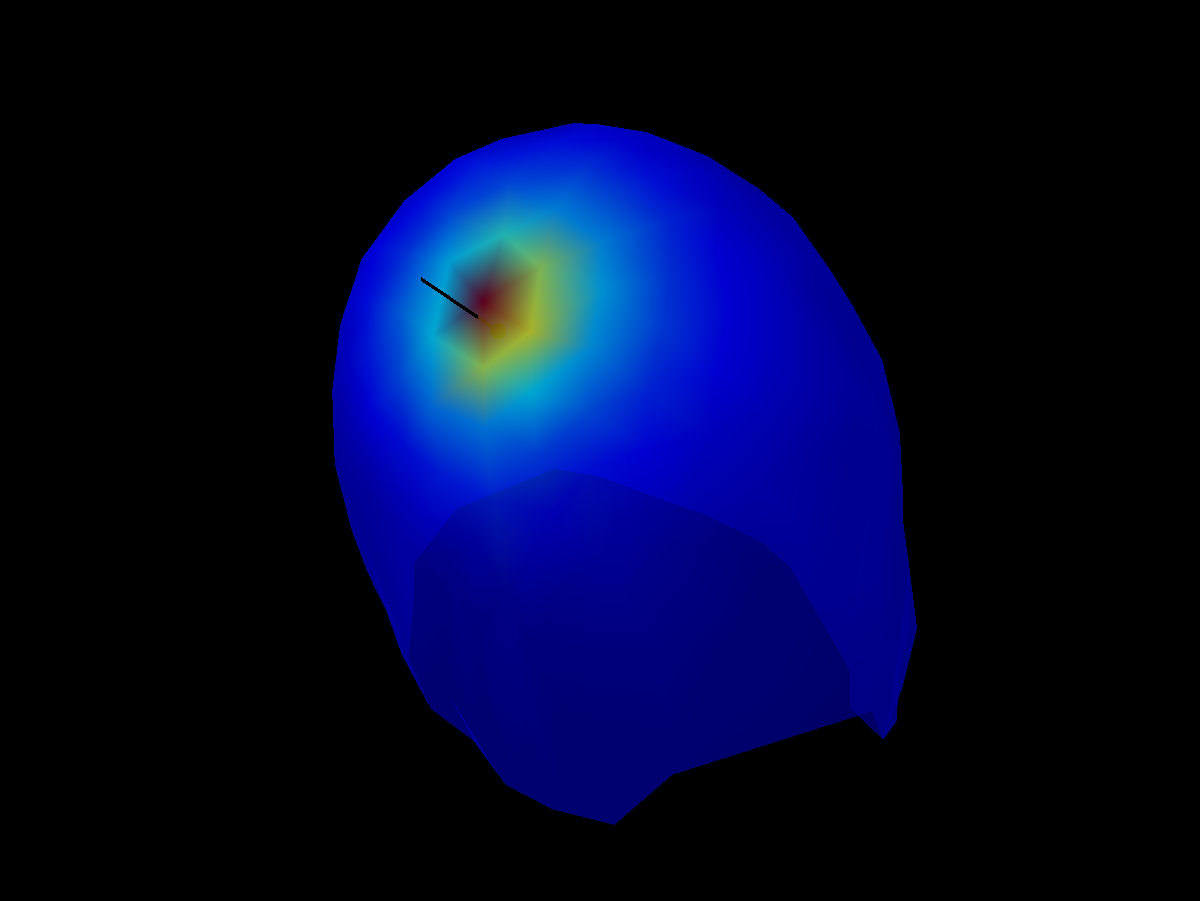
\includegraphics[width=1.2\textwidth]{./img/dipole-leadfield-radial-superficial-2.png}

\end{column}

\begin{column}{3.5cm}
\begin{flushright}
summation
\end{flushright}
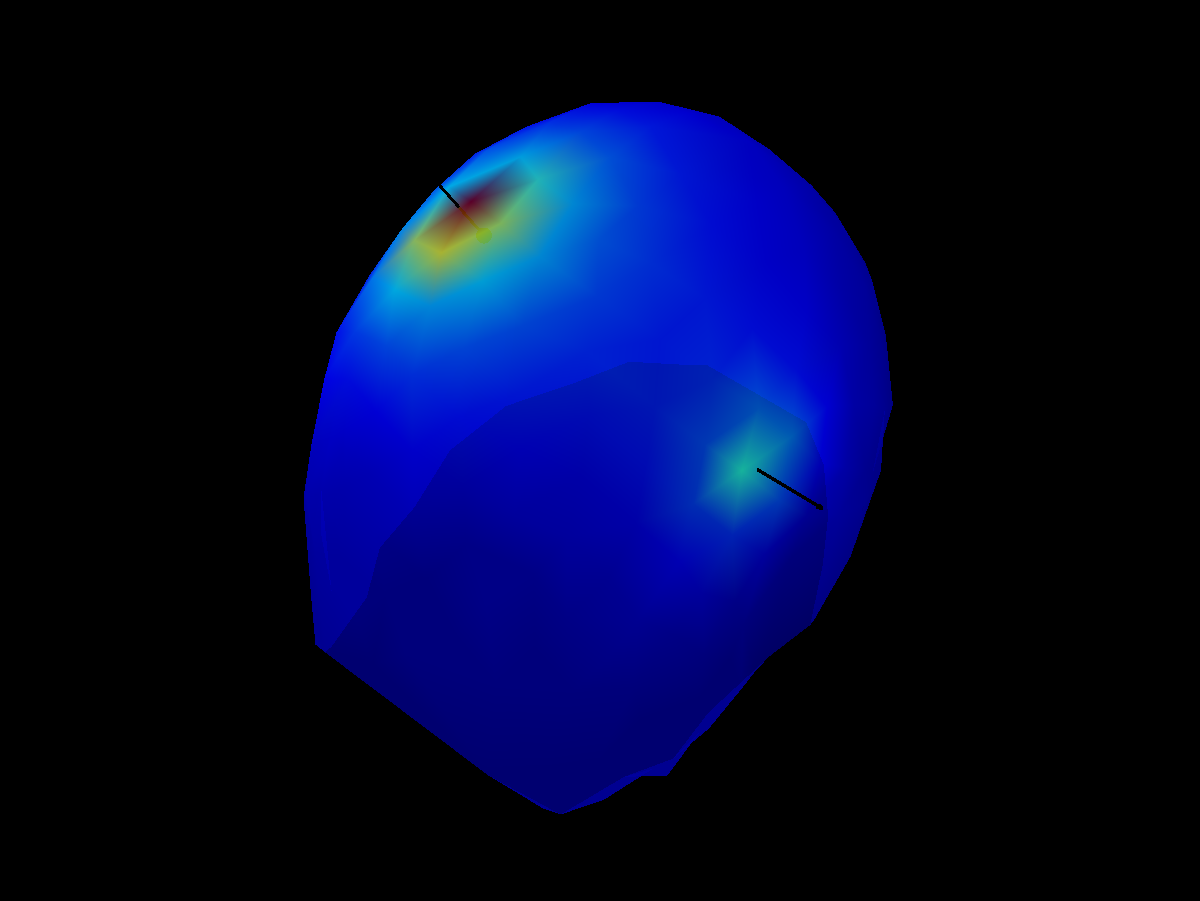
\includegraphics[width=1.3\textwidth]{./img/dipole-leadfield-summation.png}

\end{column}


\end{columns}



}


%%%%%%%%%%%%%%%%%%%%%%%%%%%%%%%%%%%%%%%%%%%%%%%%%%%%%% SPHERICAL HEAD MODELS


\frame{\frametitle{Spherical head models}

\begin{itemize}
\item One or several concentric spheres with constant (but possibly anisotropic conductivity) 
\vspace{.1cm}
\item For single-shell isotropic head models, the forward problem can be solved analytically
\vspace{.1cm}
\item For multi-shell (possibly anisotropic) spherical head models you can use Berg's equivalent dipoles method
\end{itemize}

\begin{center}
\begin{figure}
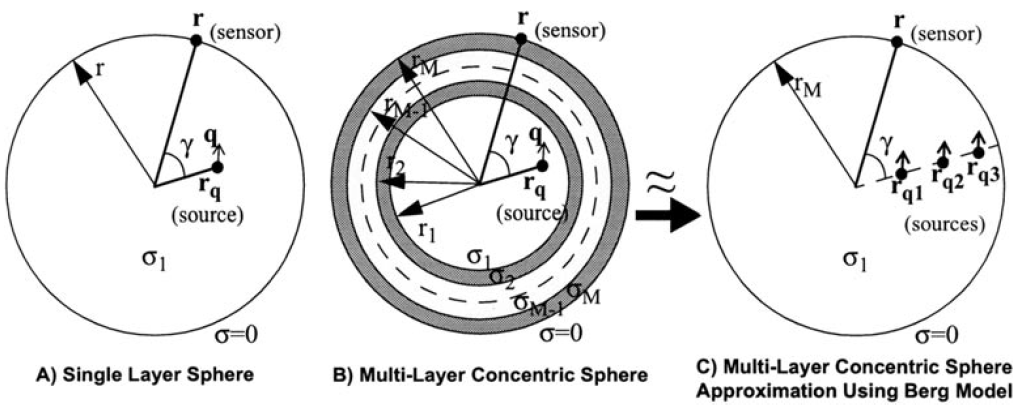
\includegraphics[width=.7\textwidth]{./img/berg.png}
\end{figure}
\ssmall{From: Ermer et al., Phys. Med. Biol., 2001}
\end{center}

}

%%%%%%%%%%%%%%%%%%%%%%%%%%%%%%%%%%%%%%%%%%%%%%%%%%%%%%% BERG'S EQUIVALENT DIPOLES METHOD
%
%\frame{\frametitle{Berg's equivalent dipoles method}
%
%\begin{itemize}
%\item Approximates a single dipole multi-shell spherical head model with a 3-dipole single-shell model
%\vspace{.5cm}
%\item Forward fields are additive
%\vspace{.5cm}
%\item The single-shell forward model can be solved analytically
%\end{itemize}
%\begin{columns}
%\begin{column}{.6\textwidth}
%\begin{block}{Multishell models and their Berg dipoles}
%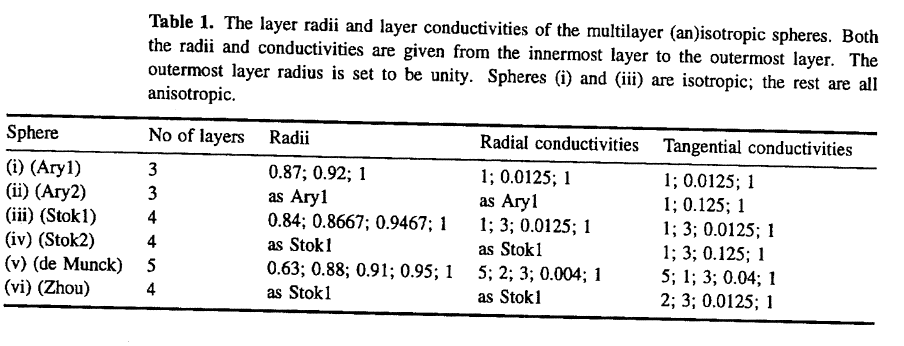
\includegraphics[width=\textwidth]{./img/zhang-table.png}
%\end{block}
%\end{column}
%\begin{column}{.4\textwidth}
%\ssmall{From: Zhang, Phys. Med. Biol., 1995}
%\end{column}
%\end{columns}
%
%}


%%%%%%%%%%%%%%%%%%%%%%%%%%%%%%%%%%%%%%%%%%%%%%%%%%%%%% PROBLEMS WITH SPHERICAL HEAD MODELS

\frame{\frametitle{Problems with spherical head models}

\begin{itemize}
\item Single (multi-layer) sphere models greatly distort the true sensor-dipole spatial geometry
\vspace{.2cm}
\item Sensor-weighted models with multiple spheres complicate things (too much)
\end{itemize}

\begin{center}
\begin{figure}
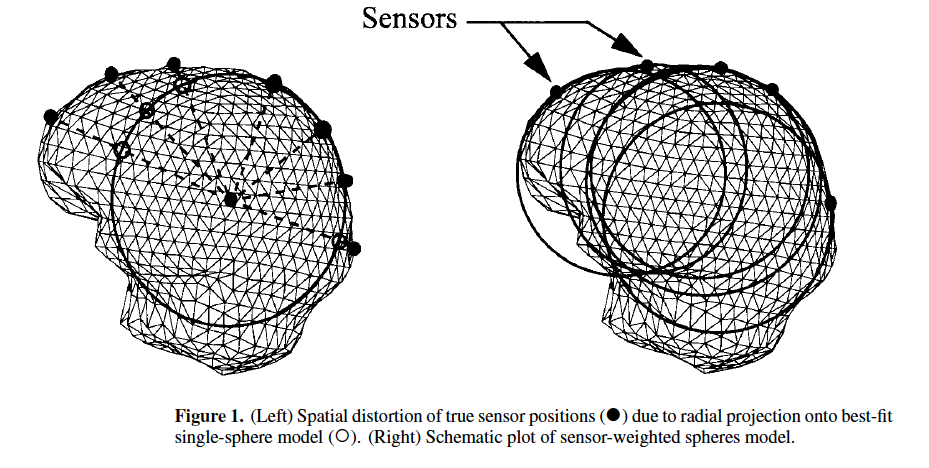
\includegraphics[width=.8\textwidth]{./img/problems-spherical.png}
\end{figure}
\ssmall{From: Ermer et al., Phys. Med. Biol., 2001}
\end{center}

}


% By its very shape, the spherical model distorts the true distribution of passive currents in the
% brain, skull and scalp. Spherical models also require that the sensor positions be projected onto
% the fitted sphere (figure 1) resulting in a distortion of the true sensor�dipole spatial geometry
% and ultimately the computed surface potential. The use of a single best-fitted multilayer sphere
% has the added drawback of incomplete coverage of the inner skull region, often ignoring areas
% such as the frontal cortex. In practice, this problem is typically resolved by fitting additional
% spheres to those regions not covered by the primary sphere. The use of these additional
% spheres results in added complication in the EEG forward model, since a neural source may
% be simultaneously inside of some spheres and outside others.



%%%%%%%%%%%%%%%%%%%%%%%%%%%%%%%%%%%%%%%%%%%%%%%%%%%%%% REALISTIC HEAD MODELS

\frame{\frametitle{Realistic head models}

\begin{itemize}
\item A realistically shaped head model can be easily constructed based on a high-quality anatomical MRI scan
\vspace{.4cm}
\item Not anymore possible to use analytical approximations, we have to rely on numerical methods
\vspace{.4cm}
\item Two numerical methods for solving the forward problem:
\begin{itemize}	
\item Boundary Element Method: isotropic tissue conductivity
\vspace{.2cm}
\item Finite Element Method
\end{itemize}
\end{itemize}


}

% It is not anymore possible to use analytical approximations, we have to rely on numerical methods



%%%%%%%%%%%%%%%%%%%%%%%%%%%%%%%%%%%%%%%%%%%%%%%%%%%%%% HEAD MODELING EXAMPLE


\frame{\frametitle{Head modeling example}


\begin{columns}
\begin{column}{.4\textwidth}
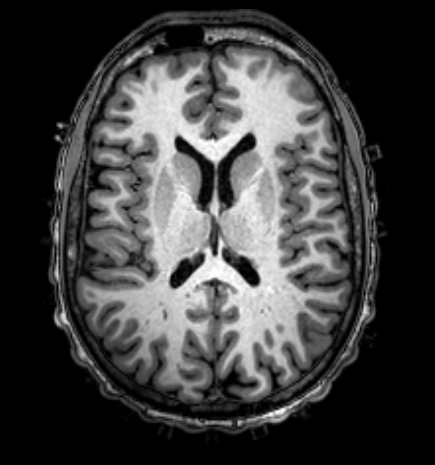
\includegraphics[width=.9\textwidth]{./img/mri.png}
\end{column}
\begin{column}{.6\textwidth}
\includegraphics<1>[width=1\textwidth,trim=2.5cm 2.5cm 2.5cm 2.5cm,crop]{./img/inner-skull.png}
\includegraphics<2>[width=1\textwidth,trim=2.5cm 2.5cm 2.5cm 2.5cm,crop]{./img/outer-skull.png}
\includegraphics<3>[width=1\textwidth,trim=2.5cm 2.5cm 2.5cm 2.5cm,crop]{./img/outer-skin.png}
\includegraphics<4>[width=1\textwidth,trim=2.5cm 2.5cm 2.5cm 2.5cm,crop]{./img/outer-skin-sensors.png}
\end{column}
\end{columns}



}





%%%%%%%%%%%%%%%%%%%%%%%%%%%%%%%%%%%%%%%%%%%%%%%%%%%%%%%%%%%%%%%%% SECTION: INVERSE PROBLEM


\section{The inverse problem}
\subsection*{}




%%%%%%%%%%%%%%%%%%%%%%%%%%%%%%%%%%%%%%%%%%%%%%%%%%%%%% FROM FORWARD TO INVERSE: FITTING THE DATA

\frame{\frametitle{From forward to inverse: fitting the data}


\begin{columns}
	\begin{column}{.3\textwidth}
	\begin{center}
	Observations
	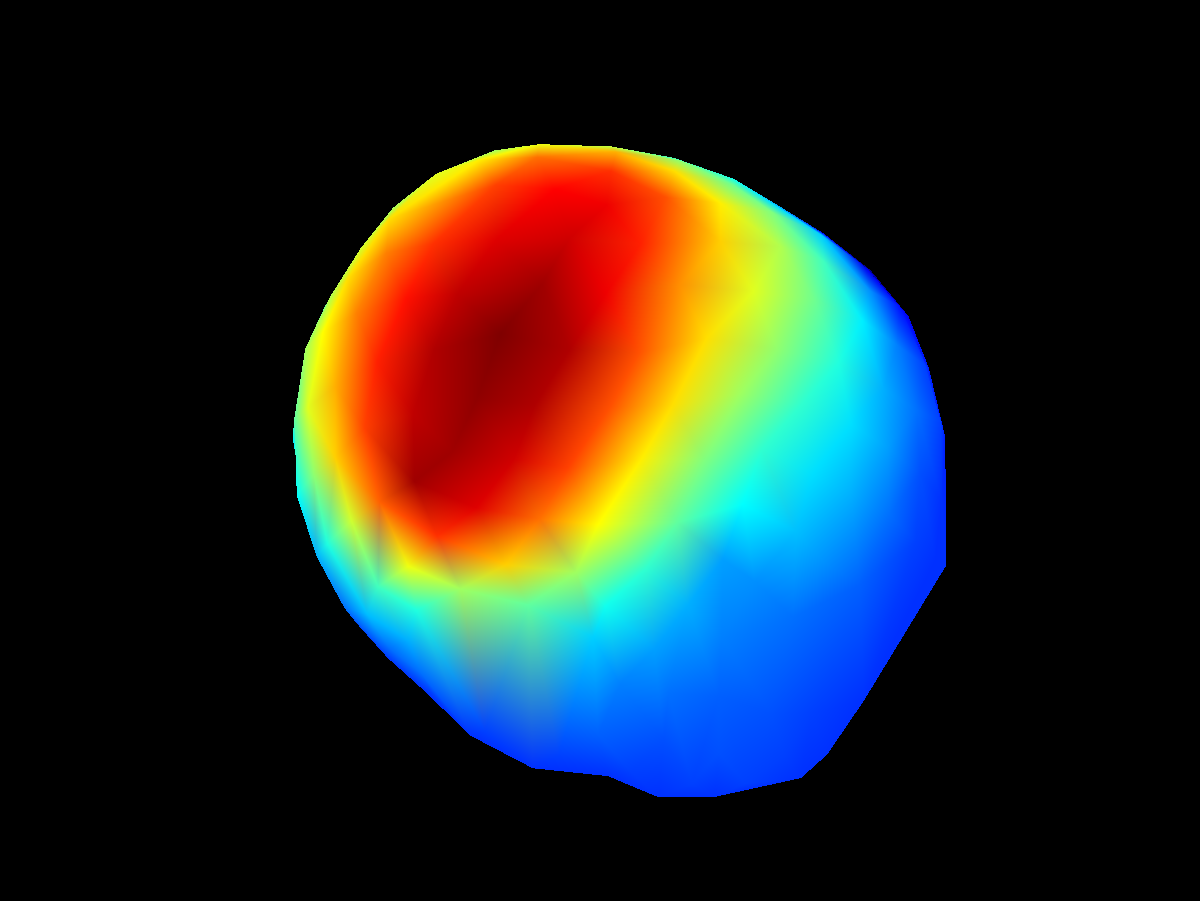
\includegraphics[width=\textwidth,trim=1cm 0cm 0cm 0cm,crop]{./img/observations.png}
	\end{center}
	\end{column}
	
	\begin{column}{.1\textwidth}
	\Huge{-}
	\end{column}
	
	\begin{column}{.3\textwidth}
	\begin{center}
	Model
	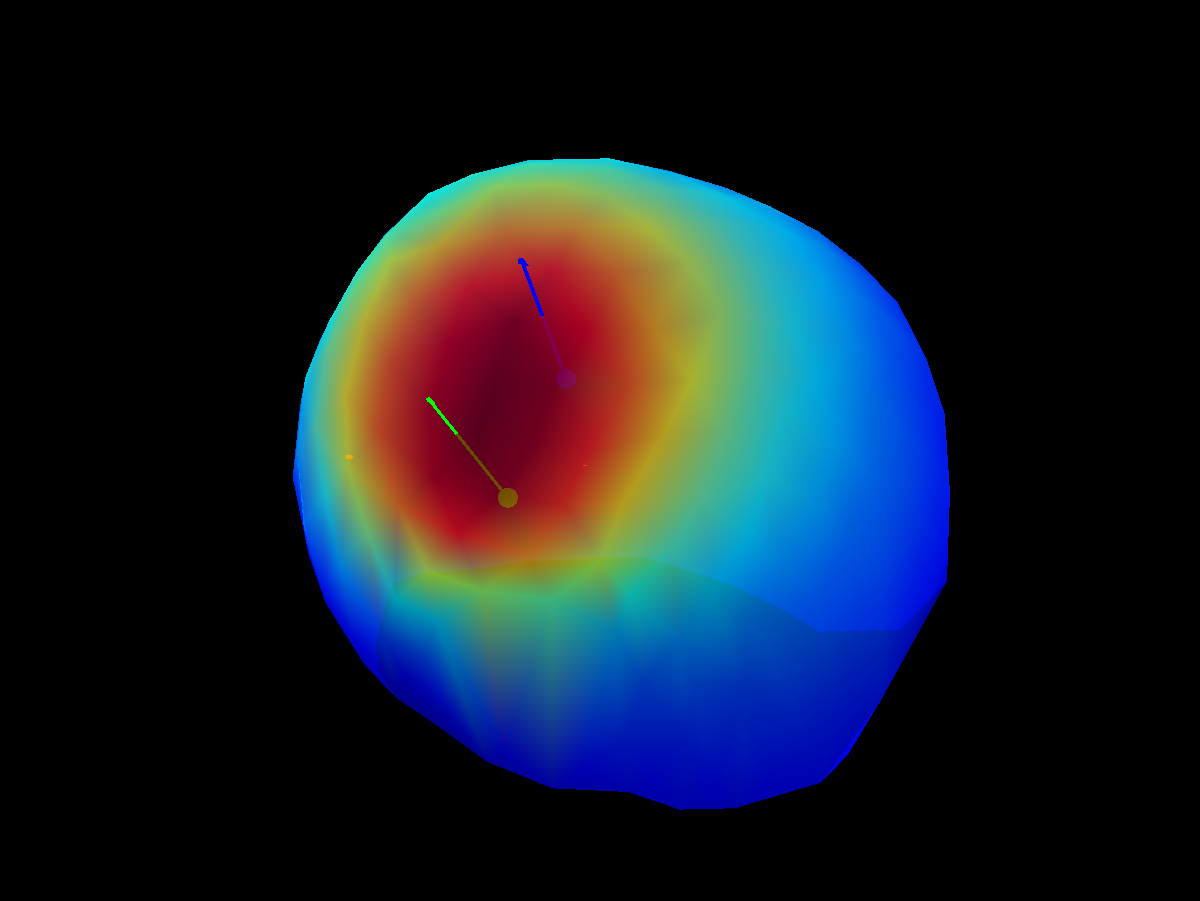
\includegraphics[width=\textwidth,trim=1cm 0cm 0cm 0cm,crop]{./img/model.png}
	\end{center}
	\end{column}
	
	\begin{column}{.1\textwidth}
	\Huge{=}
	\end{column}

	\begin{column}{.3\textwidth}
	\begin{center}
	Residuals
	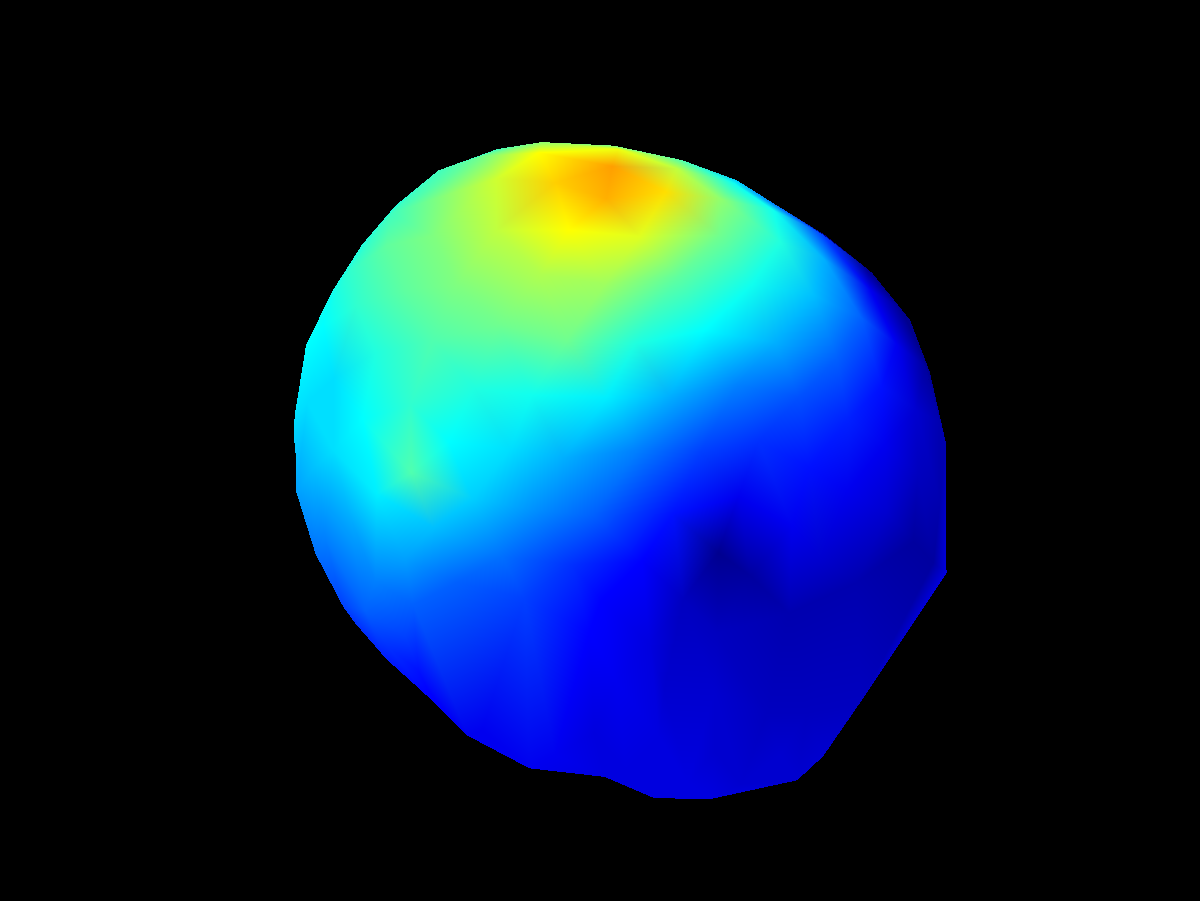
\includegraphics[width=\textwidth,trim=1cm 0cm 0cm 0cm,crop]{./img/residuals.png}
	\end{center}
	\end{column}
\end{columns}

\vspace{1cm}

\alert{Goal:} Adjust model parameters in order to minimize the difference between source model and observed data

}


%%%%%%%%%%%%%%%%%%%%%%%%%%%%%%%%%%%%%%%%%%%%%%%%%%%%%% THE INVERSE SOLUTION IS NOT UNIQUE 

\frame{\frametitle{Major caveat: the inverse solution is not unique}

\begin{itemize}
\item Fitting perfectly the data does not necessarily mean that our model matches the true underlying sources
\vspace{.3cm}
\item The solution to the M/EEG inverse problem is not unique
\vspace{.3cm}
\item However, few solutions are compatible with constraints from:
\begin{itemize}
\item Electrophysiology and cortical anatomy
\item Cross-condition and cross-subjects inferences
\item Multi-modal investigations (MEG+EEG+fMRI+...)
\end{itemize}
\vspace{.3cm}
\item \alert{Our M/EEG inverse solution is nothing more than a model!}
\end{itemize}

}


%%%%%%%%%%%%%%%%%%%%%%%%%%%%%%%%%%%%%%%%%%%%%%%%%%%%%% TWO MAIN CLASSES OF INVERSE SOLVERS


\frame{\frametitle{Two main classes of inverse solvers}
	
	\begin{columns}
		\begin{column}{.5\textwidth}
		
		\begin{center}
		Localization approach
		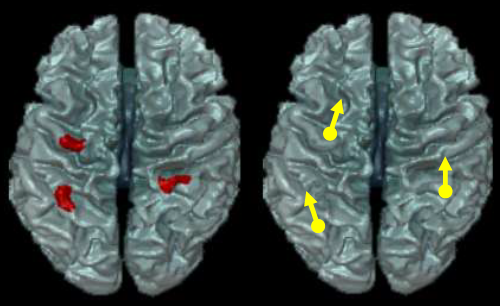
\includegraphics[width=.7\textwidth]{./img/localization.png}
		\end{center}
		\begin{itemize}
		\item Equivalent Current Dipoles
		\item An overdetermined problem: Least-squares
		\item \alert{Where are the dipoles?}
		\item \alert{How many dipoles?}
		\end{itemize}
		
		\end{column}
		\begin{column}{.5\textwidth}
		\begin{center}
		\vspace{.4cm}
		Distributed approach
		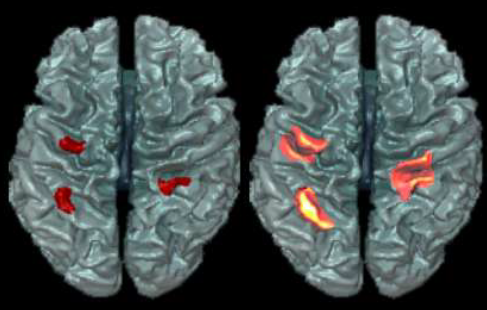
\includegraphics[width=.67\textwidth]{./img/distributed.png}
		\end{center}
		\begin{itemize}
		\item A large grid of candidate source locations
		\item \alert{How strong the sources are?}
		\item An \emph{underdetermined problem}: Minimum norm
	     \end{itemize}

		\end{column}
	
	
	\end{columns}	
	
	}



%%%%%%%%%%%%%%%%%%%%%%%%%%%%%%%%%%%%%%%%%%%%%%%%%%%%%% FEW EQUATIONS


\frame{\frametitle{Few equations}

An elementary current dipole $\vec{q}$ is fully defined by its location ($\vec{r}_q$), its magnitude (a scalar $m$) and its orientation ($\Theta=\left\{\theta,\phi\right\}$). \\
\vspace{.3cm}
The  electric potential generated by such elementary dipole at a scalp location $\vec{r}$ is given by:

\begin{columns}
\begin{column}{.6\textwidth}
\[
v(\vec{r}) = a(\vec{r},\vec{r}_q,\Theta)m
\]
\hspace{.3cm} where $a$ is a \alert{gain coefficient}
\end{column}

\begin{column}{.4\textwidth}
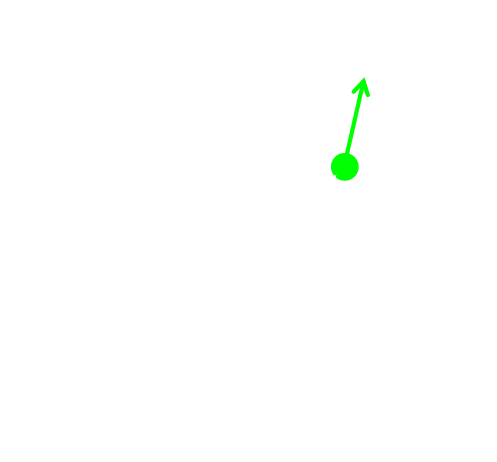
\includegraphics[width=.9\textwidth]{./img/dipole-formulas.png}
\end{column}
\end{columns}
	

}


\frame{\frametitle{Few equations}

Recall the formula of the potential generated by a dipole:
\vspace{.2cm}
\begin{center}
\boxed{
v(\vec{r}) = a(\vec{r},\vec{r}_q,\Theta)m
}
\end{center}

Generalizing the equation to $R$ dipoles and $K$ sensors is trivial:

\[
\left[
\begin{array}{c}
v_1\\
v_2\\
\vdots\\
v_K\\ 
\end{array}
\right]
= 
\underbrace{
\left[
\begin{array}{ccc}
a_{11} & \cdots & a_{1R}\\
\vdots & \ddots & \vdots\\
a_{K1} & \cdots & a_{KR}\\
\end{array}
\right]}_{\textrm{leadfield matrix: } \A}
\left[
\begin{array}{c}
m_1\\
\vdots\\
m_R\\
\end{array}
\right]
\]



}




%%%%%%%%%%%%%%%%%%%%%%%%%%%%%%%%%%%%%%%%%%%%%%%%%%%%%% EQUIVALENT CURRENT DIPOLES

\frame{\frametitle{Equivalent Current Dipoles (ECD)}

The ECD approach simply tries to minimize the following least-squares contrast:

\[
J_{LS}\left(\{\r_{qi},\Theta_i\},\m \right) = \left\|\v-\A(\{\r_{qi},\Theta_i\})\m\right\|^2
\]

which is equivalent to:
\vspace{.2cm}
\begin{center}
\boxed{
J_{LS}\left(\{\r_{qi},\Theta_i\} \right) = \left\|\v-\A\A^+\v\right\|^2
}
\end{center}

Problems:

\begin{itemize}
\item Number of dipoles has to be fixed a priori
\item A nonlinear (multivariate) optimization problem
\item Nonconvexity increases rapidly with the number of dipoles
\end{itemize}

	

}



%%%%%%%%%%%%%%%%%%%%%%%%%%%%%%%%%%%%%%%%%%%%%%%%%%%%%% DISTRIBUTED APPROACHES


\frame{\frametitle{Distributed techniques: aka Imaging approaches}

\begin{itemize}	
\item Determining the dipoles' location/orientation is difficult
	
\vspace{.2cm}
	
\item Once done that, estimating dipole amplitudes is easy
\end{itemize}
\vspace{.5cm}	
	
So...
	
\vspace{.5cm}
	
\begin{itemize}	
\item Let's place dipoles everywhere in the brain
	
\vspace{.2cm}
	
\item Let's then estimate the dipole amplitudes
	
\vspace{.2cm}
	
\item A close-to-zero amplitude would then mean the absence of a dipole at the corresponding location
\end{itemize}
	
}


%%%%%%%%%%%%%%%%%%%%%%%%%%%%%%%%%%%%%%%%%%%%%%%%%%%%%% DEFINING THE SOURCE SPACE


\frame{\frametitle{Defining the source space}
	
	\begin{itemize}
	\item Obviously, we cannot put dipoles just ''everywhere'', but we have to choose a discrete number of spatial locations: the \alert{source space} 
	\vspace{.2cm}
	\item Ideally, the source space should be based on anatomical constraints
	\vspace{.2cm}
	\item But we could also just sample uniformly the whole brain volume
	\end{itemize}
	

}


%%%%%%%%%%%%%%%%%%%%%%%%%%%%%%%%%%%%%%%%%%%%%%%%%%%%%% DIFFERENT WAYS OF DEFINING THE SOURCE SPACE


\frame{\frametitle{Different ways of defining the source space}
	
\begin{columns}
\begin{column}{.6\textwidth}
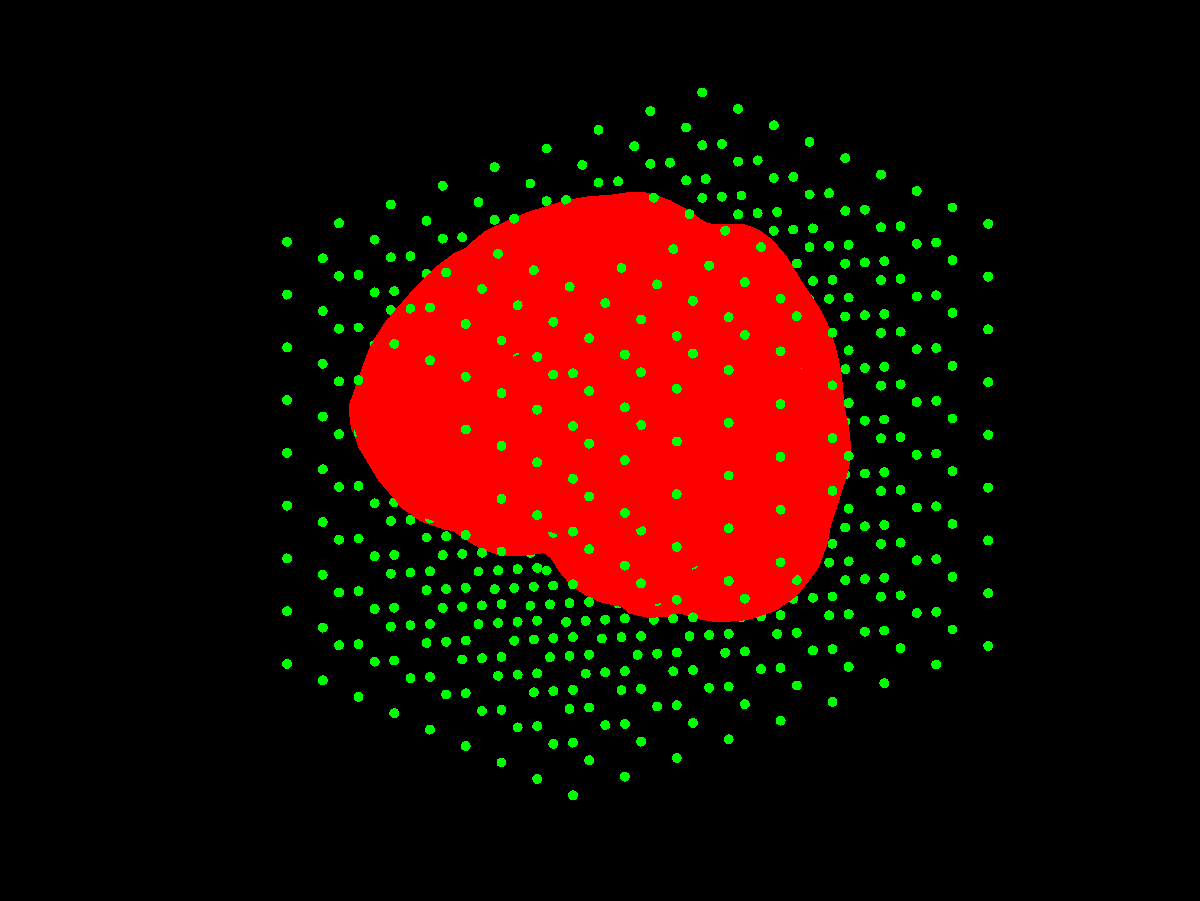
\includegraphics[width=\textwidth]{./img/source-grid-1.png}
\end{column}
\begin{column}{.4\textwidth}
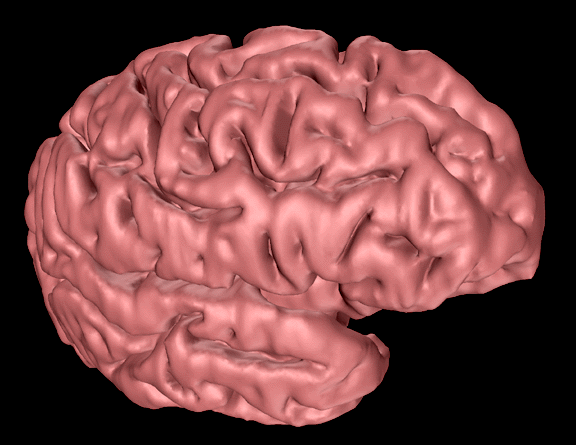
\includegraphics[width=.9\textwidth]{./img/cortical-surface.png}
\end{column}
\end{columns}	

}





%%%%%%%%%%%%%%%%%%%%%%%%%%%%%%%%%%%%%%%%%%%%%%%%%%%%%% FORMULATING THE INVERSE PROBLEM


\frame{\frametitle{Formulating the inverse problem}

For distributed approaches, we have that:

\[
\v = \A\m
\]

where $\v=[v_1, ..., v_K]^T$ are the potentials measured at $K$ scalp locations, $\A$ is a $KxR$ leadfield matrix, and $\m=[m_1, \cdots, m_R]^T$ are the magnitudes of the $R>>K$ dipoles contained in the source space.

\vspace{.2cm}

The goal now is  to minimize the contrast:

\[
J(\m) = \left\|\v-\A\m\right\|^2
\]	

\vspace{1cm}

\tiny{Note: $\left\|\z\right\|^2$ is the squared $l^2$ norm of vector $\z = [z_1, ..., z_K]$, which is defined as $\left\|\z\right\|^2 = \z_1^2+...+\z_K^2$}

}

%%%%%%%%%%%%%%%%%%%%%%%%%%%%%%%%%%%%%%%%%%%%%%%%%%%%%% DISADVANTAGES OF DISTRIBUTED APPROACHES


\frame{\frametitle{Disadvantages of distributed approaches}

\begin{itemize}
\item A heavily underdetermined inverse problem
\vspace{.3cm}
\item How to define the source space?
\vspace{.3cm}
\item How to define the boundaries between differentiated sources?
\end{itemize}
}

%%%%%%%%%%%%%%%%%%%%%%%%%%%%%%%%%%%%%%%%%%%%%%%%%%%%%% SOLUTION TO THE DISTRIBUTED INVERSE PROBLEM


\frame{\frametitle{Solution to the distributed inverse problem}

The minimum of the contrast that we showed in the previous slide is:

\[
\hat{\m}=\W\W^T\A^T\left(\A\W\W^T\A^T+\lambda\I\right)^{-1}\v
\]

where:

\vspace{.2cm}

$\A$ is the leadfield matrix

\vspace{.2cm}

$\W$ encodes a-priori information on the inverse solution

\vspace{.2cm}

$\lambda$ is a regularization parameter  
	

}



%%%%%%%%%%%%%%%%%%%%%%%%%%%%%%%%%%%%%%%%%%%%%%%%%%%%%% MINIMUM NORM ESTIMATE (MNE)


\frame{\frametitle{Minimum Norm Estimate (MNE)}

The MNE solution does not use a-priori information, so that the solution becomes:

\[
\hat{\m}=\A^T\left(\A\A^T+\lambda\I\right)^{-1}\v
\]


\begin{itemize}
\item The simplest solution
\vspace{.1cm}
\item Produces a solution $\hat{\m}$ of minimum norm 
\vspace{.1cm}
\item It favours superficial dipoles versus deeper ones, as the latter would require higher energies (i.e. norms) to account for the same amount of observed data variance
\vspace{.1cm}
\item Mostly used in combination with cortical surface models
\end{itemize}

	

}


%%%%%%%%%%%%%%%%%%%%%%%%%%%%%%%%%%%%%%%%%%%%%%%%%%%%%% THE REGULARIZATION PARAMETER


\frame{\frametitle{The regularization parameter}

Recall the MNE solution:

\[
\hat{\m}=\A^T\left(\A\A^T+\lambda\I\right)^{-1}\v
\]

Matrix $\A\A^T$ is often close to \emph(singular), i.e. hardly invertible. 

\vspace{.5cm}

The reason for this is that the leadfield matrix $\A$ is \alert{ill-conditioned}, which means that the columns of  $\A$ are not linearly independent from each other (see the lecture on fundamental linear algebra).

}


%%%%%%%%%%%%%%%%%%%%%%%%%%%%%%%%%%%%%%%%%%%%%%%%%%%%%% THE LEADFIELD MATRIX IS ILL-CONDITIONED... SO WHAT?


\frame{\frametitle{The leadfield matrix is ill-conditioned... so what?}

\begin{itemize}
\item If you ignore the ill-conditioning of the leadfield, your inverse solution will be dominated by noise
\vspace{.2cm}
\item The downside is a reduction in spatial resolution
\end{itemize}
\vspace{.5cm}
\begin{columns}
\begin{column}{.1\textwidth}
\end{column}
\begin{column}{.4\textwidth}
\ssmall No noise, good conditioning
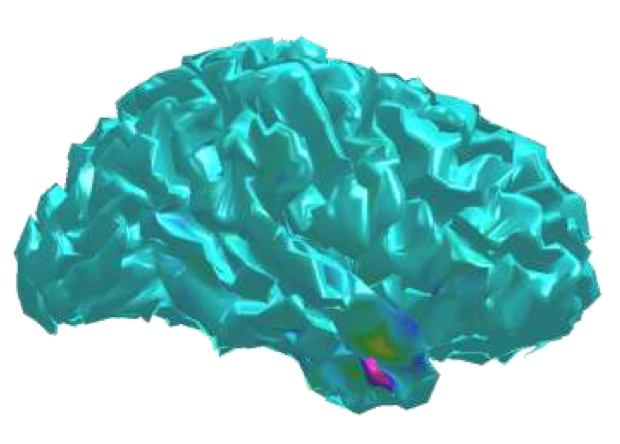
\includegraphics[width=.6\textwidth,trim=.1cm .1cm 0cm 0cm,clip]{./img/good-condition-no-noise.png}
\end{column}
\begin{column}{.4\textwidth}
\ssmall No noise, poor conditioning
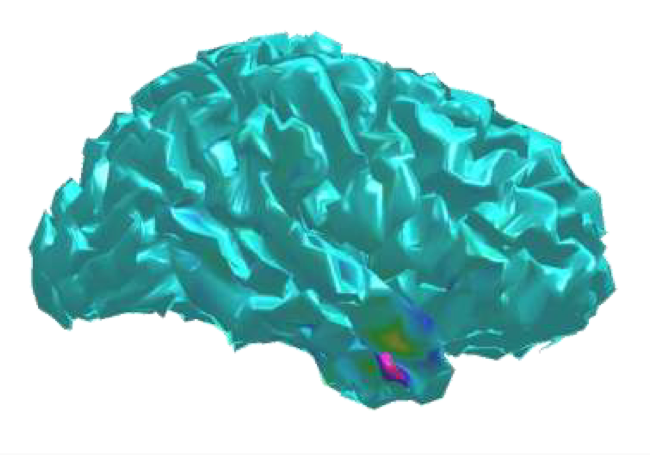
\includegraphics[width=.6\textwidth,trim=.1cm .1cm 0cm 0cm,clip]{./img/bad-condition-no-noise.png}
\end{column}
\end{columns}
\vspace{.5cm}
\begin{columns}
\begin{column}{.1\textwidth}
\end{column}
\begin{column}{.4\textwidth}
\ssmall 1\% noise, good conditioning
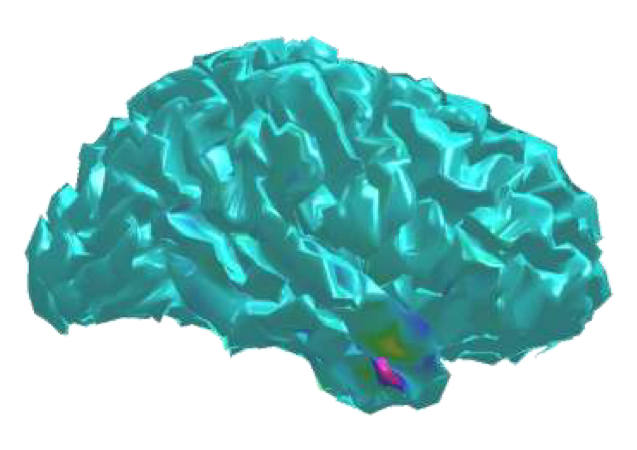
\includegraphics[width=.6\textwidth,trim=.1cm .1cm 0cm 0cm,clip]{./img/good-condition-noise.png}
\end{column}
\begin{column}{.4\textwidth}
\ssmall 1\% noise, poor conditioning
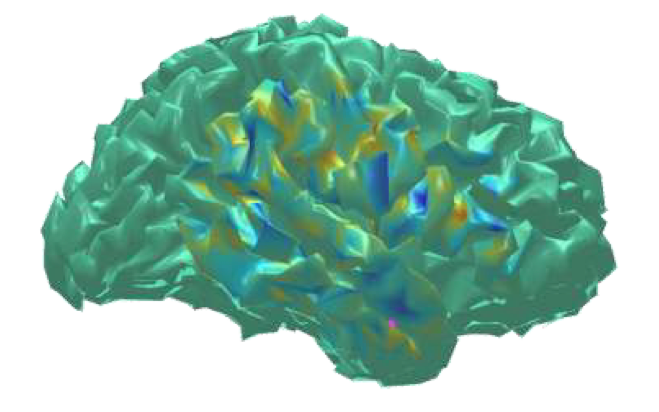
\includegraphics[width=.6\textwidth,trim=.1cm .1cm .6cm 0cm,clip]{./img/bad-condition-noise.png}
\end{column}
\end{columns}

\vspace{.3cm}
\hspace{1cm}\tiny{Figures from: Baillet, 2010, http://hbmpresentersdirectory.org}

}


%%%%%%%%%%%%%%%%%%%%%%%%%%%%%%%%%%%%%%%%%%%%%%%%%%%%%%%%%%%%%%%%% SECTION: DO WE NEED INVERSE MODELING?

\section{Do we need inverse modeling?}
\subsection*{}

\frame{
\frametitle{The sleep slow oscillation as a traveling wave}
\begin{center}
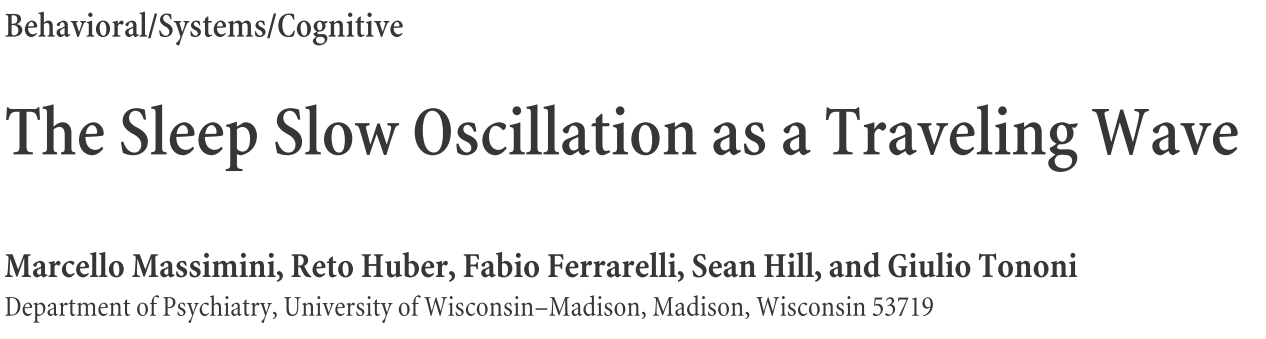
\includegraphics[width=.9\textwidth]{./img/massimini-title.png}
\end{center}

\begin{itemize}
\item ''..each oscillation is a traveling wave that periodically sweeps the cerebral cortex with a definite site of origin and a pattern of propagation''
\item Propagation speed is constant ($\sim$ 2.6 m/s)
\item ''...the wave starts small and then waxes and wanes''
\item The direction of propagation is preferentially anteroposterior
\end{itemize}
}

\frame{
\frametitle{Massimini et al.'s observations}

\begin{center}
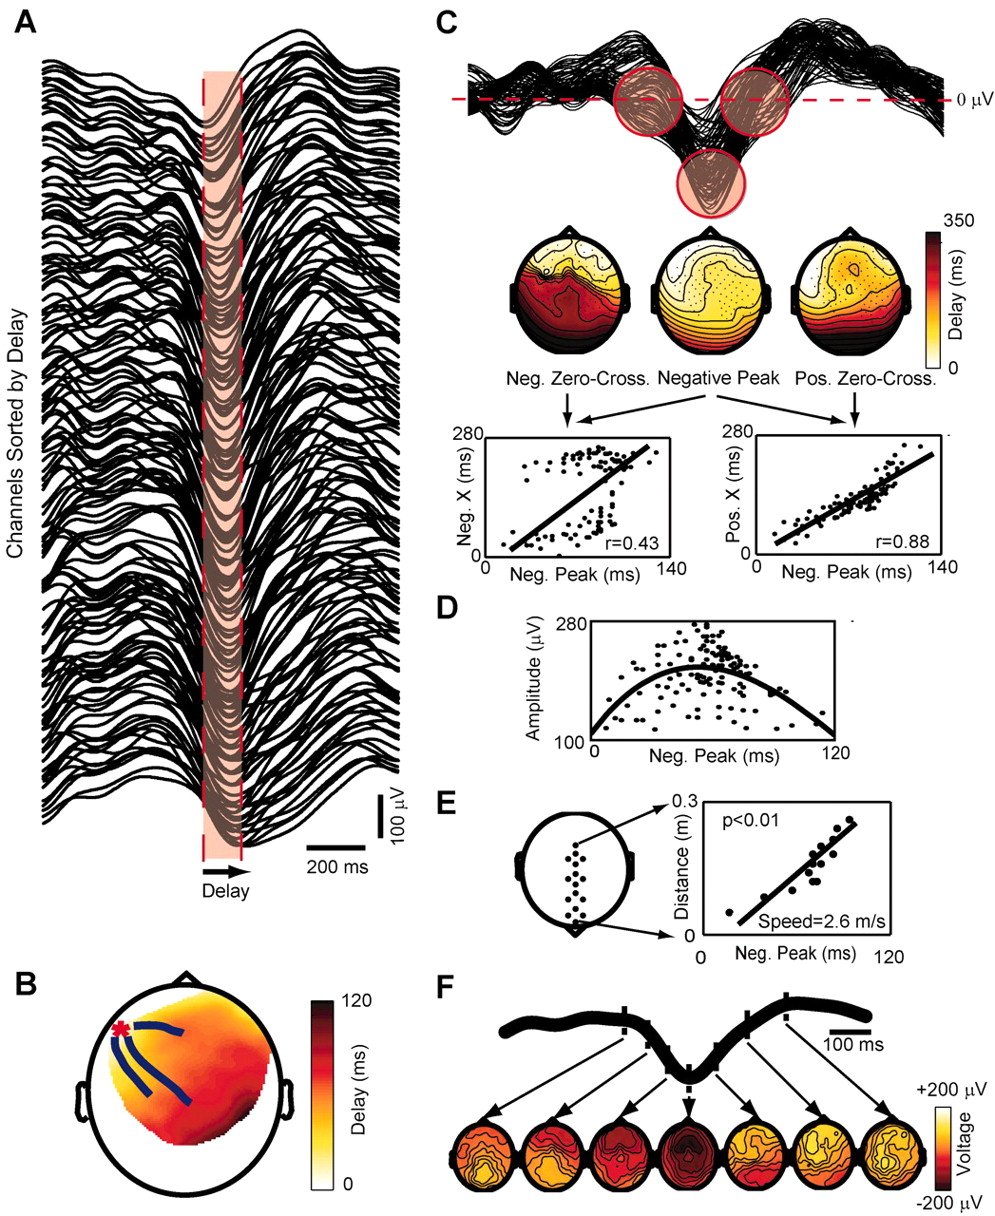
\includegraphics[height=.8\textheight]{./img/massimini-fig1.jpeg}
\end{center}

}

%%%%

\frame{
\frametitle{Simulated EEG sources in fixed locations}

\begin{center}
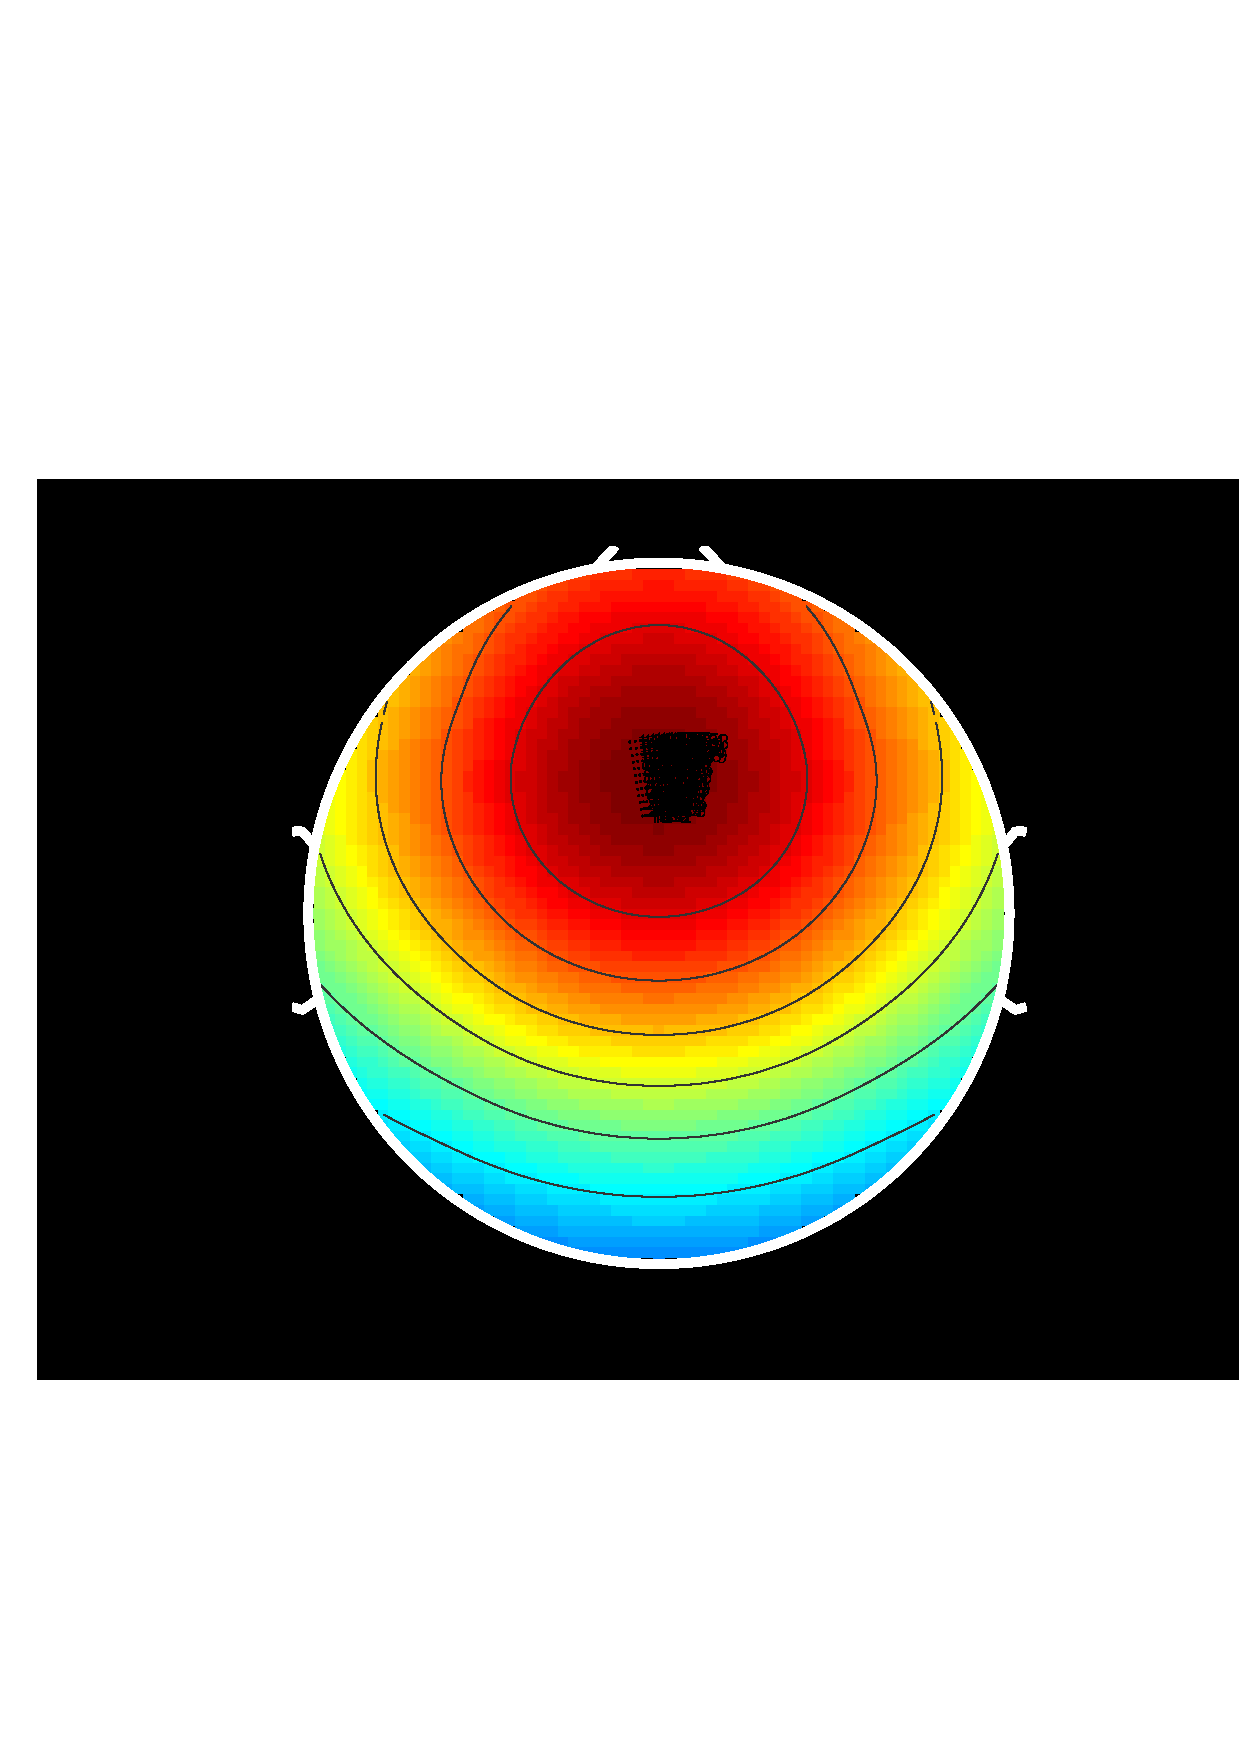
\includegraphics[width=.5\textwidth,trim = 1cm 5cm 2cm 8cm,clip]{./img/fig-massimini-anterior.pdf}
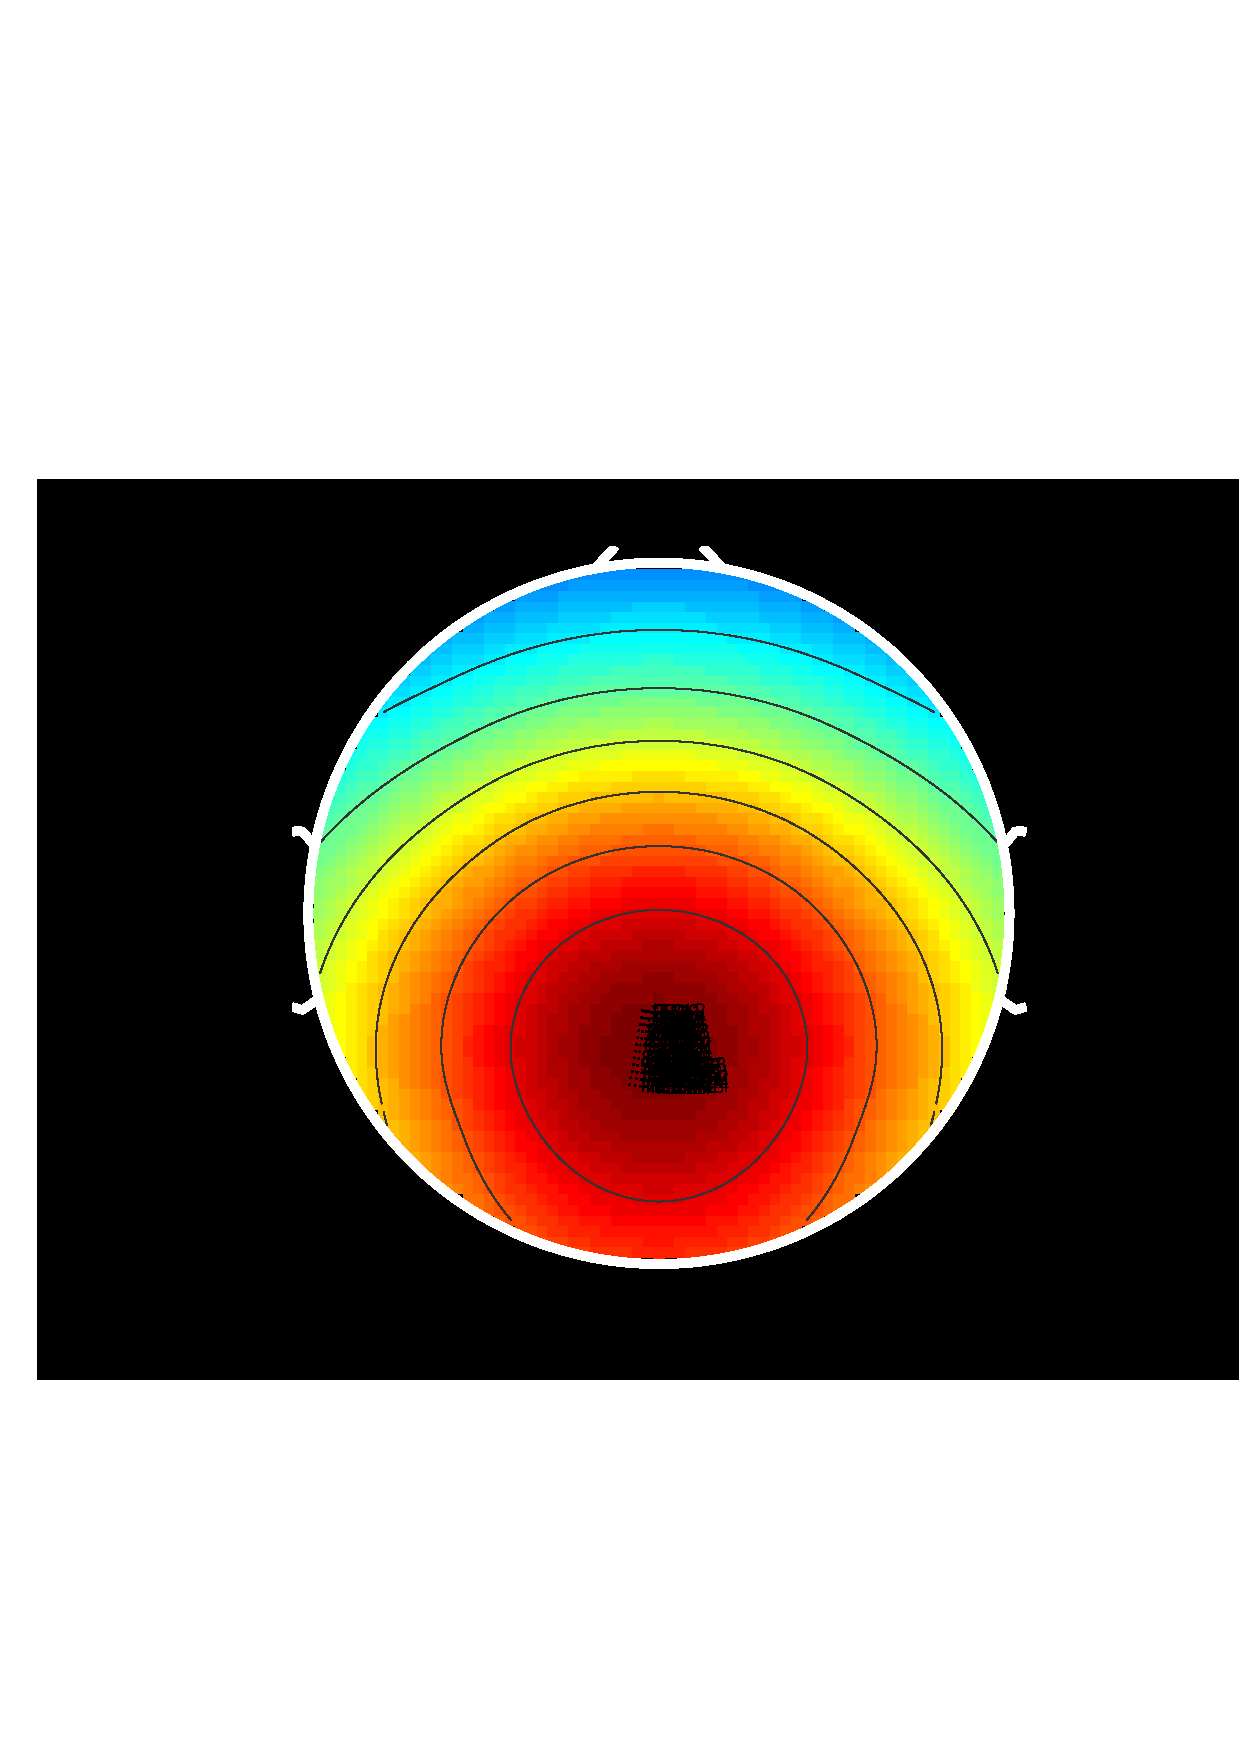
\includegraphics[width=.5\textwidth,trim = 1cm 5cm 2cm 8cm,clip]{./img/fig-massimini-posterior.pdf}
\end{center}

}

%%%%%%%%%%%%%%%%%%%%%%%%%%%%%%%%%%%%%%%%%%%%%%%%%%%%%%%%%%%%%%%%%%%%%%%%%%%%%%%%%%%%%%%%%%

\frame{
\frametitle{Topography vs time}

\begin{block}{A traveling wave?}
\begin{center}
\animategraphics[autoplay,loop,width=7cm]{5}{./animated/massimini/frame}{1}{20}
\end{center}
\end{block}

}



%%%%%%%%%%%%%%%%%%%%%%%%%%%%%%%%%%%%%%%%%%%%%%%%%%%%%%%%%%%%%%%%%%%%%%%%%%%%%%%%%%%%%%%%%%

\frame{
\frametitle{Wave speed and amplitude}

\begin{center}
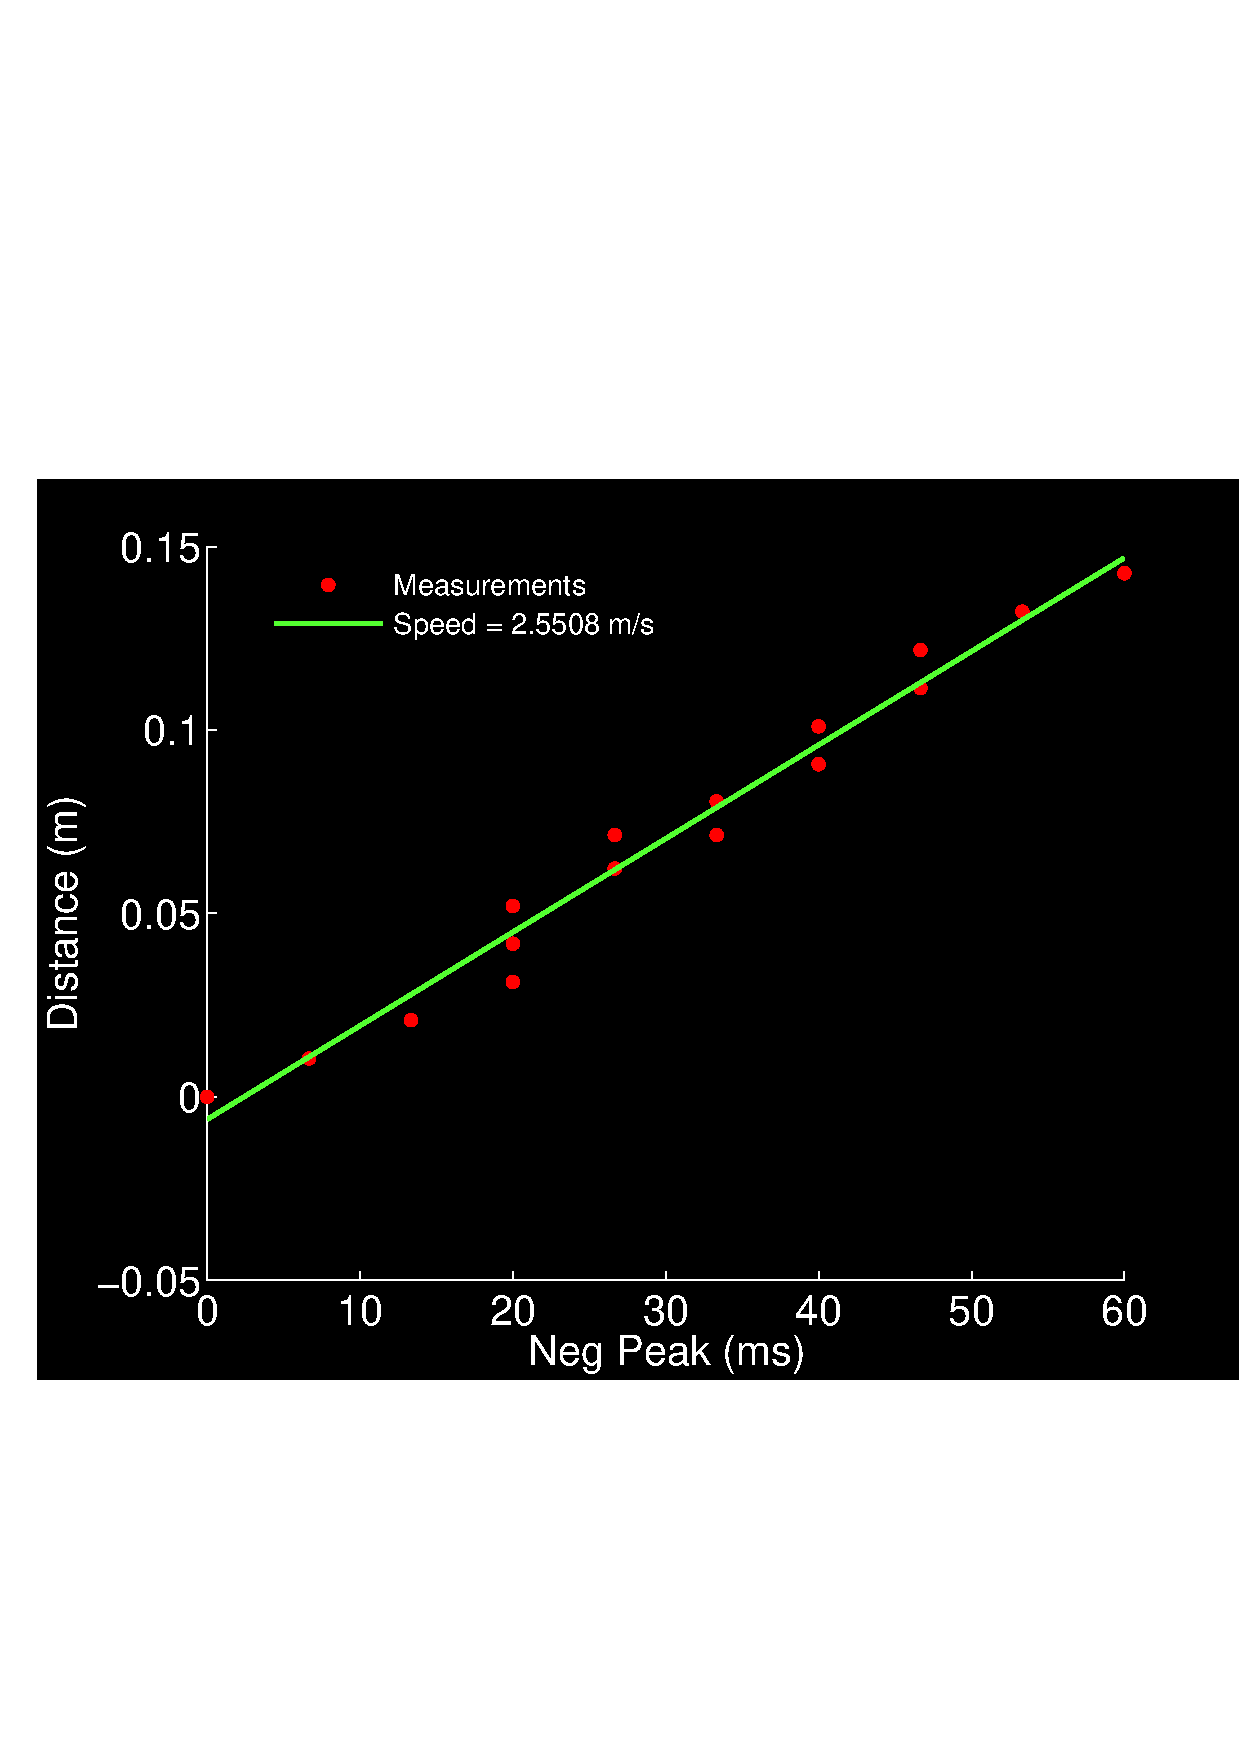
\includegraphics[width=.5\textwidth,trim = 0cm 5cm 1cm 8cm,clip]{./img/fig-massimini-speed.pdf}
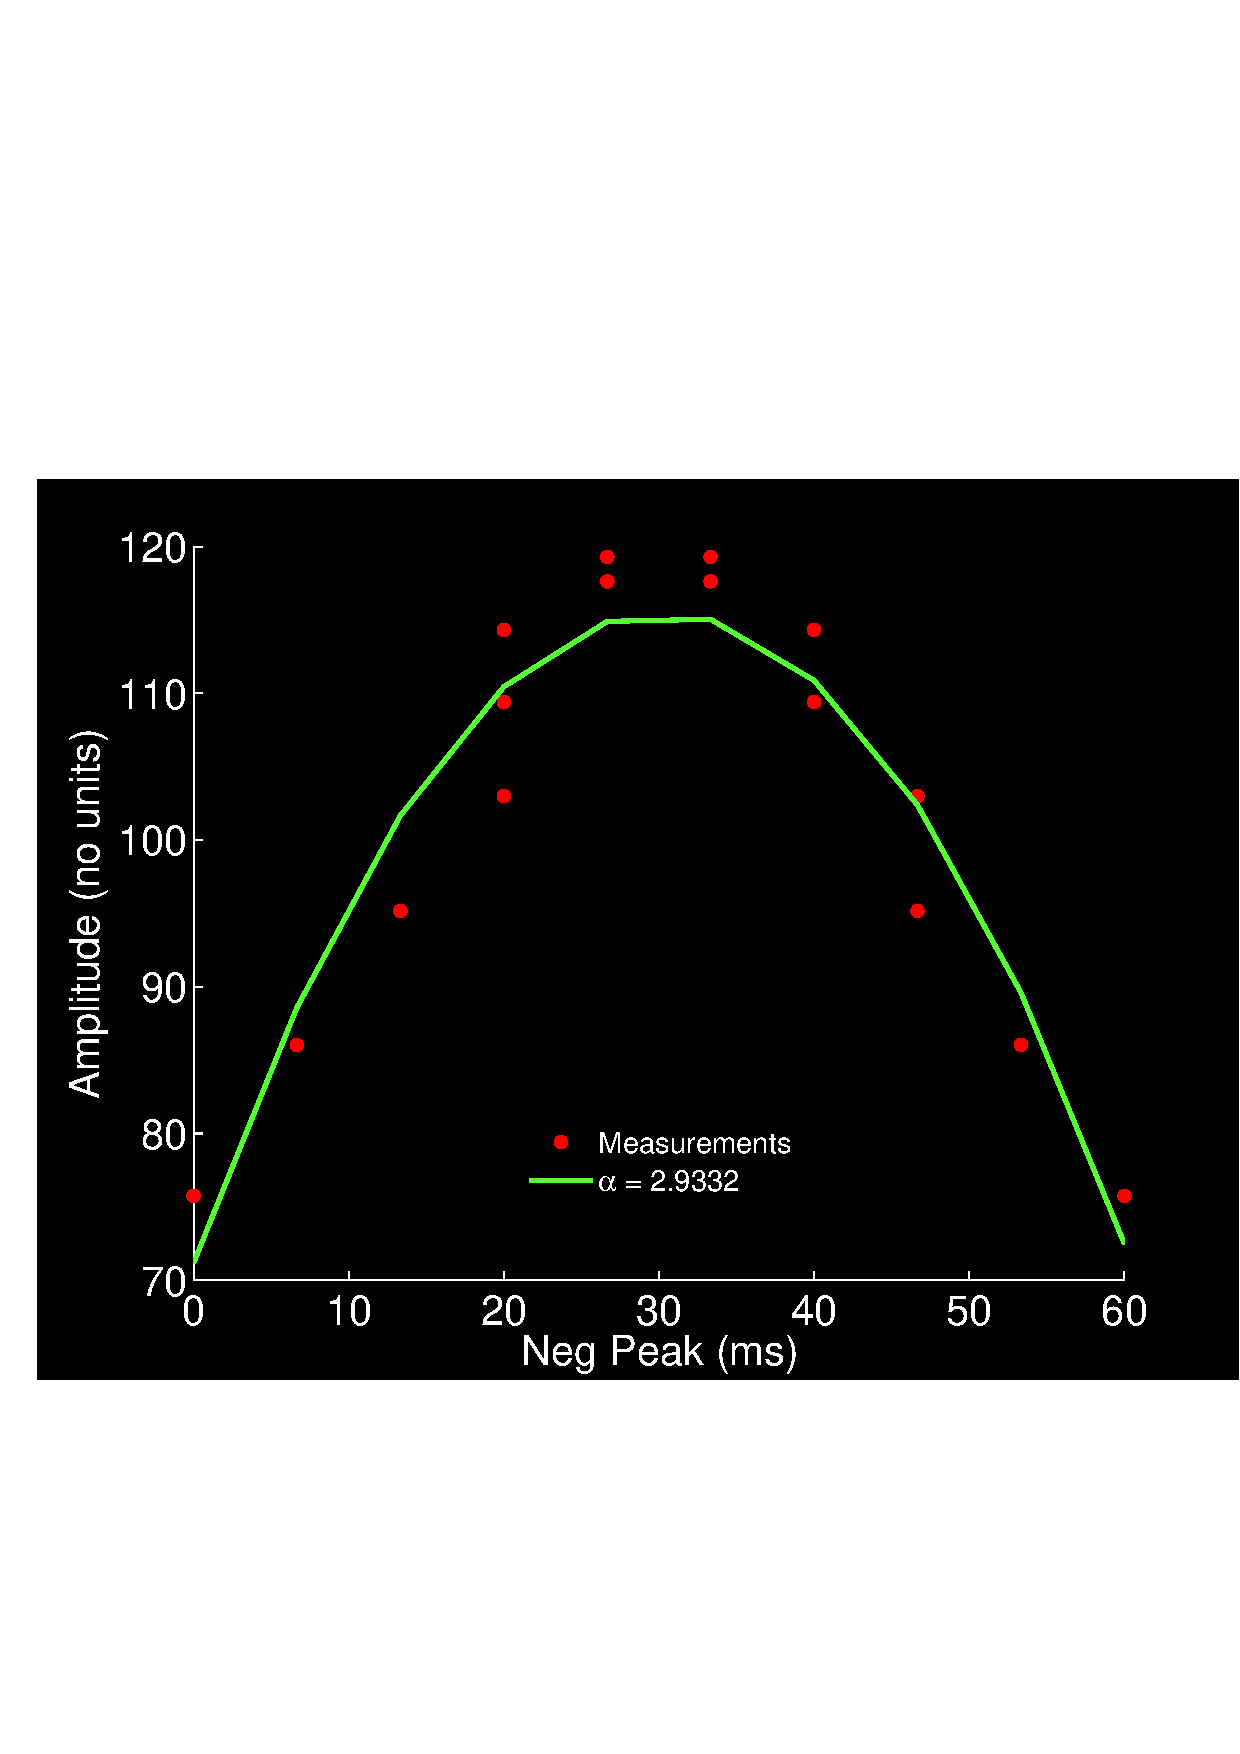
\includegraphics[width=.5\textwidth,trim = 0cm 5cm 1cm 8cm,clip]{./img/fig-massimini-amplitude.pdf}
\end{center}

}




%%%%%%%%%%%%%%%%%%%%%%%%%%%%%%%%%%%%%%%%%%%%%%%%%%%%%%%%%%%%%%%%% SECTION: INVERSE PROBLEM


\section{Key points}
\subsection*{}


%%%%%%%%%%%%%%%%%%%%%%%%%%%%%%%%%%%%%%%%%%%%%%%%%%%%%% KEY POINTS


\frame{\frametitle{Key points}
	\begin{itemize}
	\item The main cerebral generators of the EEG are synchronously activated large pyramidal cortical neurons
	\vspace{.2cm}
	\item The spatial resolution of M/EEG is fundamentally limited by the ambiguity of the inverse problem
	\vspace{.2cm}
	\item For M/EEG frequencies, the forward electromagnetic model reduces to a linear and instantaneous mapping
	\vspace{.2cm}
	\item Spherical head models allow for approximate analytical solutions of the forward problem (Berg's method)
	\vspace{.2cm}
	\item Realistic head models require numerical methods for solving the forward problem: BEM or FEM
	\end{itemize}

}

%%%%%%%%%%%%%%%%%%%%%%%%%%%%%%%%%%%%%%%%%%%%%%%%%%%%%% SLIDE 27


\frame{\frametitle{Key points (cont'd)}

\begin{itemize}
\item Single (multi-layer) sphere models are the simplest but can greatly distort the sensor-dipole spatial geometry
\vspace{.2cm}
\item Inverse solvers aim to adjust model parameters (dipole locations/orientations/magnitudes) in order to minimize the difference between source model and observed data
\vspace{.2cm}
\item Fitting the observed data alone does not guarantee an accurate inverse solution: additional constraints based on anatomy, a-priori knowledge, multimodal imaging, etc... are very recommendable
\end{itemize}
	
}

\frame{\frametitle{Key points (cont'd)}

\begin{itemize}
\item The main disadvantages of ECDs approach to the inverse problem are ....
\vspace{.2cm}
\item The main disadvantages of distributed approaches are ....
\vspace{.2cm}
\item What is the problem introduced by an ill-conditioned leadfield matrix?
\vspace{.2cm}
\item What technique can be used to overcome an ill-conditioned leadfield matrix? What is the downside of such technique?
\end{itemize}
	
}


%%%%%%%%%%%%%%%%%%%%%%%%%%%%%%%%%%%%%%%%%%%%%%%%%%%%%% REFERENCES AND ATTRIBUTION:


\frame{\frametitle{References and attribution:}


These slides are partially based on this article:

\vspace{.5cm}

(Baillet et al., 2001) Electromagnetic Brain Mapping, IEEE Signal Processing Magazine

\vspace{1cm}

A tutorial on the topic of this presentation is available at:

\vspace{.5cm}

\url{http://kasku.org/tutorials/tutorial_dipoles}

}



\end{document}